\documentclass[12pt,a4paper]{report}

\usepackage{float} % for table float: Alex
\usepackage{multirow} % for table
\usepackage{mathtools} % pentru formule: Alex
\usepackage[section]{placeins} % tabele sa stea in sectiunea lor: Alex
\usepackage{listings} % pentru cod sursa: Alex
\usepackage{svg}

\usepackage[utf8]{inputenc} % pentru suport diacritice
\usepackage[english]{babel} % setări pentru limba română 
\renewcommand\familydefault{\sfdefault} % sans serif

\usepackage[margin=2.54cm]{geometry}	% dimensiuni pagină și margini
\usepackage{graphicx} % support the \includegraphics command and options

% formatting sections and subsections
\usepackage{textcase}
\usepackage[titletoc, title]{appendix}
\usepackage{titlesec}
\titleformat{\chapter}{\large\bfseries\MakeUppercase}{\thechapter}{2ex}{}[\vspace*{-1.5cm}]
\titleformat*{\section}{\large\bfseries}
\titleformat*{\subsection}{\large\bfseries}
\titleformat*{\subsubsection}{\large\bfseries}

\usepackage{chngcntr}
\counterwithout{figure}{chapter} % no chapter number in figure labels
\counterwithout{table}{chapter} % no chapter number in table labels
\counterwithout{equation}{chapter} % no chapter number in equation labels

\usepackage{booktabs} % for much better looking tables
\usepackage{url} % Useful for inserting web links nicely
\usepackage[bookmarks,unicode,hidelinks]{hyperref}

\usepackage{array} % for better arrays (eg matrices) in maths
\usepackage{paralist} % very flexible & customisable lists (eg. enumerate/itemize, etc.)
\usepackage{verbatim} % adds environment for commenting out blocks of text & for better verbatim
\usepackage{subfig} % make it possible to include more than one captioned figure/table in a single float
\usepackage{enumitem}
\setlist{noitemsep}

%%% HEADERS & FOOTERS
\usepackage{fancyhdr}
\pagestyle{empty}
\renewcommand{\headrulewidth}{0pt}
\renewcommand{\footrulewidth}{0pt}
\lhead{}\chead{}\rhead{}
\lfoot{}\cfoot{\thepage}\rfoot{}



\newcommand{\HeaderLineSpace}{-0.25cm}
\newcommand{\UniTextRO}{UNIVERSITATEA POLITEHNICA DIN BUCUREȘTI \\[\HeaderLineSpace] 
FACULTATEA DE AUTOMATICĂ ȘI CALCULATOARE \\[\HeaderLineSpace]
DEPARTAMENTUL DE CALCULATOARE\\}
\newcommand{\DiplomaRO}{PROIECT DE DIPLOMĂ}
\newcommand{\AdvisorRO}{Coordonator științific:}
\newcommand{\BucRO}{BUCUREȘTI}

\newcommand{\UniTextEN}{UNIVERSITY POLITEHNICA OF BUCHAREST \\[\HeaderLineSpace]
FACULTY OF AUTOMATIC CONTROL AND COMPUTERS \\[\HeaderLineSpace]
COMPUTER SCIENCE AND ENGINEERING DEPARTMENT\\}
\newcommand{\DiplomaEN}{DIPLOMA PROJECT}
\newcommand{\AdvisorEN}{Thesis advisor:}
\newcommand{\BucEN}{BUCHAREST}

\newcommand{\frontPage}[5]{
\begin{titlepage}
\begin{center}
{\Large #1}  % header (university, faculty, department)
\vspace{50pt}
\begin{tabular}{p{6cm}p{4cm}}

\includegraphics[scale=0.8]{pics/upb-logo.jpg} &
	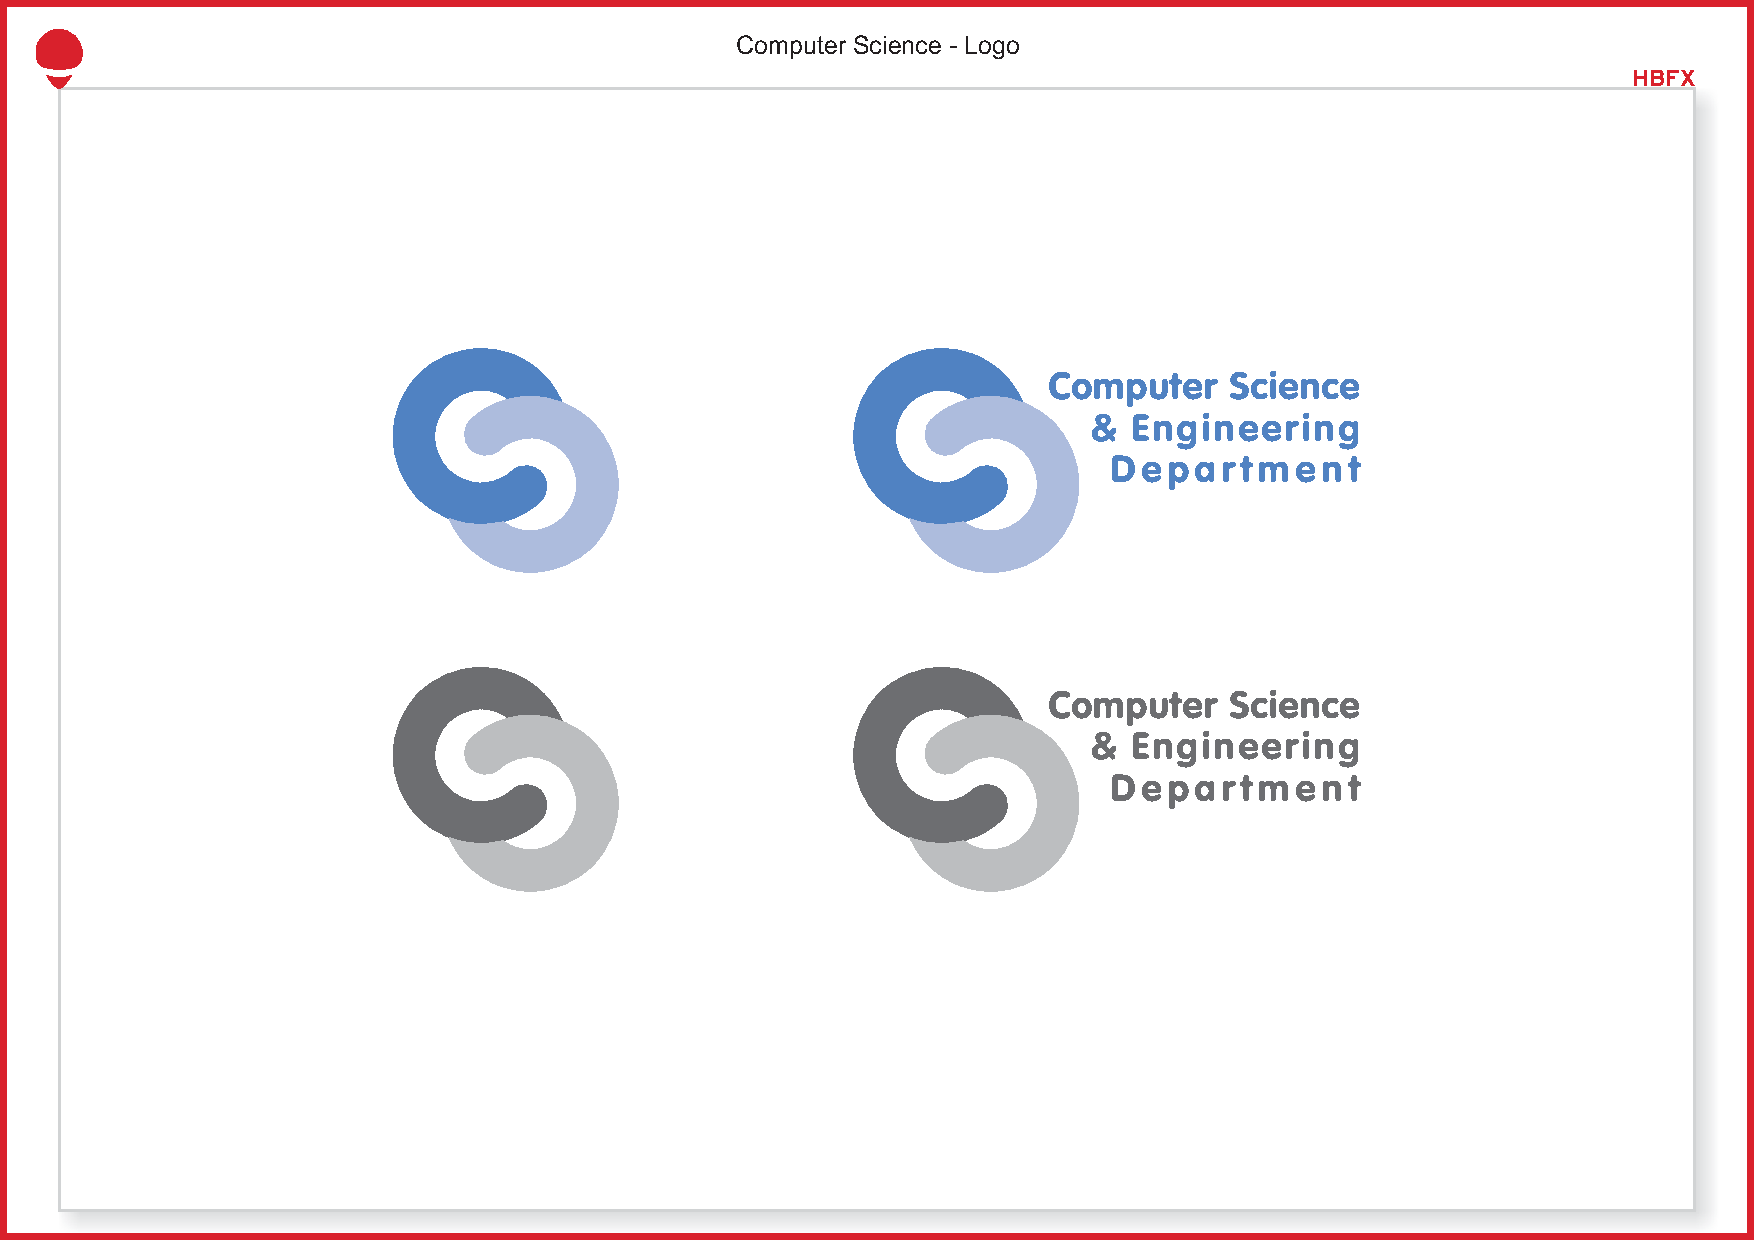
\includegraphics[scale=0.5,trim={14cm 11cm 2cm 5cm},clip=true]{pics/cs-logo.pdf}
\end{tabular}

\vspace{105pt}
{\Huge #2}\\                           % diploma project text
\vspace{40pt}
{\Large #3}\\ \vspace{0pt}  % project title
% {\Large #4}\\                          % project subtitle
\vspace{40pt}
{\LARGE \Name}\\                   % student name
\end{center}
\vspace{60pt}
\begin{tabular*}{\textwidth}{@{\extracolsep{\fill}}p{6cm}r}
&{\large\textbf{#4}}\vspace{10pt}\\      % scientific advisor
&{\large \Advisor}\\                                    % advisor name
&{\large \AdvisorA}\\                                    % advisor name

\end{tabular*}
\vspace{20pt}
\begin{center}
{\large\textbf{#5}}\\                                % bucharest
\vspace{0pt}
{\normalsize \Year}
\end{center}
\end{titlepage}
}

\newcommand{\frontPageRO}{\frontPage{\UniTextRO}{\DiplomaRO}{\ProjectTitleRO}{\AdvisorRO}{\BucRO}}
\newcommand{\frontPageEN}{\frontPage{\UniTextEN}{\DiplomaEN}{\ProjectTitleEN}{\AdvisorEN}{\BucEN}}

\linespread{1.15}
\setlength\parindent{0pt}
\setlength\parskip{.28cm}

%% Abstract macro
\newcommand{\AbstractPage}{
\begin{titlepage}
% \textbf{\large SINOPSIS}\par
% \AbstractRO\par\vfill
\textbf{\large ABSTRACT}\par
\AbstractEN \vfill
\end{titlepage}
}

%% Thank you macro
\newcommand{\ThanksPage}{
\begin{titlepage}
{\noindent \large\textbf{ACKNOWLEDGEMENTS}}\\
\Thanks
\end{titlepage}
}



%%%%%%%%%%%%%%%%%%%%%%%%%%%%%%%%%%%%%%%%%%%%%%%%%%   
%%
%%          End of template definitions
%%   
%%%%%%%%%%%%%%%%%%%%%%%%%%%%%%%%%%%%%%%%%%%%%%%%%%


\newcommand{\ProjectTitleRO}{Algoritm de detectare de erori de cod}
\newcommand{\ProjectSubtitleRO}{}
\newcommand{\ProjectTitleEN}{Bug Detection and Repair}
\newcommand{\ProjectSubtitleEN}{}
\newcommand{\Name}{Alexandru-Constantin Jercan}
\newcommand{\Advisor}{Conf. Dr. Ing. Traian Eugen Rebedea}
\newcommand{\AdvisorA}{Drd. Ing. Radu Cristian Alexandru Iacob}
\newcommand{\Year}{2023}

\title{Proiect de diplomă}
\author{\Name}
\date{\Year}

\newcommand{\AbstractRO}{\ldots}

\newcommand{\AbstractEN}{Software has become an essential aspect of our world. Thus, source code has attracted many researchers to apply machine learning techniques to solve tasks such as bug detection and repair. To explore this task we are going to analyze a specific area of software development, algorithmic style problems. We are going to summarize recent attempts to solve the problem and provide our approach of solving it. We are going to explore relevant datasets and see what types of bugs we encounter and how to solve them. We introduce a new dataset containing buggy and accepted submissions for algorithmic problems. Finally, we will look at our bug detection and repair pipeline that can be used for finding mistakes in Python and C++ code and suggesting fixes for them.}

\newcommand{\Thanks}{\ldots}

\begin{document}

% \frontPageRO
\frontPageEN

\begingroup
\linespread{1}
\tableofcontents
\endgroup

\AbstractPage

\chapter{Introduction}\pagestyle{fancy}

We can undoubtedly state the fact that code has become an essential aspect of the modern world. With use cases in medicine, finances, transportation and many others, software engineers are expected to develop new features and applications faster and faster. With new advancements in AI and technology there is a growing trend in using machine learning and statistics to build tools that help programmers with their work  \cite{puri2021codenet, allamanis2018survey}.

With this increased pressure to produce code quickly, it is expected that many programmers will encounter buggy or faulty source code at some point. A robust solution to minimize this issue is writing unit tests, but to maximize the users happiness and have them use the latest features, programmers will usually have to give up some of the test coverage. This is the part of a software program that would benefit from an automated way of identifying errors and minimize even further the risk of encountering bugs in code.

The problem of bug detection and code repair has become more and more popular in the last couple of years with the apparition of very powerful deep learning models such as GitHub Copilot \footnote{"GitHub Copilot · Your AI pair programmer." [Online]. Available: https://copilot.github.com/}. This tool is capable of generating syntactically correct code from the context of a file with the help of a developer's comments and sometimes incomplete instructions. What led to the success of this tool is the existence of large collections of data that can be used to train complex models. The availability of data on repository hosting platforms such as GitHub or GitLab for open source projects is huge. Looking at the history of very important open source projects, such as Linux, we can see thousand of commits and millions of changes in the source code files. Many of these changes include bug-fixes, adding new features, removing deprecated functionalities, improving the documentation and a lot more tasks. However, with this much data, also comes great responsibility, since there exists open source projects that might not follow the best practices of programming, as we have seen that it was the case for Copilot to sometimes output code instructions that were not secure \cite{pearce2021asleep}. 

Other than open source projects there are also other sources of data, for example online coding competitions, where you have to solve algorithmic style problems. With the main difference that submissions to such competitions are usually short and cover only one simple functionality, which is more often than not the contrary to most of the software development projects found online. Some other differences that we found, and maybe everyone would expect, is that solutions to competitive programming problems will not take into account using secure and up to date libraries or functions, especially when it comes to reading and writing the output to console. However, this small security issue will not shadow one of the most interesting aspects about this type of data, which is the fact that most of the failed submissions will have consecutive attempts that will, at some point, result with an accepted problem. This means that we can keep track of the submissions of one specific user and see what changes led to them making the problem work, and what bugs caused the error messages from the compiler. To have access to such data we are going to use the CodeNet project \cite{puri2021codenet} which is a large collection of competitive programming submissions and low level tools that can be used for data visualization and feature engineering. 

To make a bug fixing algorithm easier to understand we can split it in two parts, a bug detection task and an instruction suggestion task. The bug detection part has the responsibility of identifying the location of a suspicious instruction in a given file, stating what the problem with the usage of that instruction may be. And the instructions suggestion algorithm which would provide a replacement for such an instruction. We can think of the bug detection task as searching for logical errors in natural language, eg. using a word that has the wrong meaning in that sentence, the only difference being that the source code is more strict than spoken languages. And as a consequence, we can think of the instruction suggestion task as a word replacement task, but not just for grammatical errors.

In our work we have explored the possibility to solve the problem of bug detection and repair as a machine translation task, but we have also looked into more recent methods, such as using large language models. One such example is ChatGPT\footnote{https://openai.com/blog/chatgpt} which has proved to be really capable of tackling code synthesis tasks.

To summarize our contributions

\begin{enumerate}
  \item \textbf{BugNet}\footnote{https://huggingface.co/datasets/alexjercan/bugnet}. We introduce a new dataset that contains pairs of buggy-working submissions for programming problems.
  \item \textbf{AocEval}\footnote{https://huggingface.co/datasets/alexjercan/AoC/}. We introduce an evaluation dataset containing programming bugs that we used to benchmark the capabilities of large language models to repair code.
  \item \textbf{Chain of Thought}. We present a framework to use in prompting large language models to improve their ability of understanding source code. 
\end{enumerate}

\chapter{Related Work}

\section{Dataset}

\textbf{POJ-104}

The POJ-104 \cite{mou2015convolutional} dataset is a collection of source code files and only contains samples written in the C/C++ programming language. The corpus contains 52,000 correct submissions for 104 different problems. 

This dataset does not contain any submission that is rejected by the judge system. The fact that there are no samples of code that have non accepted submission status represents the greatest limitation of this dataset. This limitation is strictly related to the task that we are interested in. However, this dataset shows us that it is possible to use online judge systems to generate a dataset for source code research.

\textbf{GCJ}

The GCJ dataset contains source code samples that were submitted to the Google Code Jam competitions from 2008 to 2020. The datset contains 2,430,000 correct submissions for 332 different problems. This dataset provides a high variety of programming languages used, with 20 different ones used in solving the problems.

The GCJ dataset, however, suffers from the same limitations as POJ-104, and the missing metadata and failing source code examples will not enable us to perform bug detection on this dataset. But again we see that an even larger dataset was created by using online judge systems.

\textbf{CodeNet} 

CodeNet \cite{puri2021codenet} is a project with the objective to create a large scale dataset for source code research. To provide the best means for source code analysis it contains samples for over 50 different programming languages. With it's high variety of programming languages, the dataset contains 10 times more code samples than GCJ. 

Another feature of CodeNet is the highly annotated data. The dataset contains 13,916,868 submissions for 4053 problems which are collected from online judge web sites. The problems are annotated with the corresponding statement in Hypertext Markup Language (HTML) format. The problem statement contains a description of the problem in natural language, the problem constraints and the sample input and output.

As stated in CodeNet, a submission will refer to a source code sample that is uploaded by an user in an attempt to solve a specific problem. Intuitively, submissions will not always result in an accepted status, but sometimes in a some kind of an error. To capture this aspect, the dataset contains submission level annotations that show the result and the user that uploaded that code sample.

For machine learning tasks, the source code examples have to be independent and identically distributed (iid) to obtain reliable performance metrics \cite{10.1145/3359591.3359735}. The CodeNet dataset conforms to this rule and identifies source code samples that are near duplicates.

The extra annotations and information presented are only available in CodeNet and are missing from both POJ-104 and GCJ. This makes CodeNet a better starting point for our research.

\textbf{The Pile}

The Pile \cite{gao2020pile} dataset is an 825 GiB English text corpus collected from 22 different sources. Of interest is the GitHub subset that contains 95.16 GiB and makes up for 7.59\% of the data. The repositories used for generating the dataset are filtered to have at least 100 stars. Then the repositories are filtered only for source code. The subset is then obtained by random sampling.

\textbf{MBPP}

Mostly Basic Python Problems (MBPP) \cite{austin2021program} contains 974 short Python functions written by hand. The dataset consists of the problem statement, three test cases and one ground truth solution. In the paper it was discussed that only three test cases is enough to have a confidence of 90\% that the code generated by a language model would be semantically correct. There are also cases where the model would overfit on the test cases and generate code that only passes that.

\textbf{HumanEval}

HumanEval \cite{chen2021evaluating} is a hand-written evaluation set of 164 problems. Each problem includes a function signature, docstring, body, and several unit tests. The dataset was created to evaluate the Codex language model. The dataset contains only one solution for each problem, and the solution is implemented such that it passes all tests.

\textbf{The Stack}

The Stack \cite{Kocetkov2022TheStack} is a dataset containing 6TB of samples of source code collected from open source projects from GitHub. The dataset covers 358 programming languages. The projects and code files contained by the dataset were created between January 1st, 2015, and March 31st, 2022.

The dataset contains a feature which allows users to opt out from the dataset, and you can also check if your code if part of it \footnote{https://huggingface.co/spaces/bigcode/in-the-stack} (Fun fact, the code for my research project is also part of the stack).

\textbf{RedPajama}

The RedPajama \cite{together2023redpajama} dataset consists of 1.2 trillion tokens. The dataset is a reproduction of the training data used in the LLaMA paper. It also includes code data from GitHub, alongside natural language collected from Wikipedia and other sources.

\textbf{How is our subset different?}

Since the task we want to approach is bug detection, we want to obtain a dataset that will contain as many source code files with buggy annotated instructions as possible. From the aforementioned datasets, only CodeNet can be used to achieve this objective.

We created a subset, BugNet, which contains Python and C++ source code files. These were the most popular programming languages in the CodeNet dataset and had the most submissions made. After removing the problems that had missing or malformed metadata we are left with 65,186 submissions pairs for 3,867 different problems. This means that we have 65,186 examples of buggy source code, but also the fix for each of them.

As in the case of CodeNet, all the source code files are annotated at the submissions level. On top of this, the generated subset now also contains annotations at the chunk level. We were able to achieve this by executing each source code sample on the example input and output and parse the error to create an annotation. A chunk is a contiguous sequence of lines, or a block of code.

\begin{table}[H]\small\linespread{1}
\centering
\caption{Differentiation of related datasets}
\label{tab:relatedwork1}
\begin{tabular}{p{6cm} l >{\raggedright\arraybackslash}p{2cm} >{\raggedright\arraybackslash}p{2cm} >{\raggedright\arraybackslash}p{2cm} >{\raggedright\arraybackslash}p{1cm} >{\raggedright\arraybackslash}p{1cm}}
 & \textbf{BugNet} & \textbf{CodeNet} & \textbf{GCJ} & \textbf{POJ-104}\\
\hline Number of problems                       & 3867 & 4053 & 332 & 104 \\
\hline Number of programming languages          & 2 & 55 & 20 & 2 \\
\hline Number of code samples                   & 65,186 & 13,916,828 & 2,430,000 & 52,000 \\
\hline Percentage of problems with test data    & 100\% & 51\% & 0\% & 0\% \\
\hline Submission level error annotation        & Yes & Yes & No & No \\
\hline Chunk level error annotation              & Yes & No & No & No \\
\end{tabular}
\end{table}

We built the BugNet subset to be able to use it in the task of bug detection. We filtered only the problems that contained full metadata, in the cases of statement, constraints and input/output examples. In this case we have all the source code samples testable, at least with the example input and output. Since we created a subset of CodeNet we inherited many of the properties it provided, such as the submission level error annotation. Finally, our contribution to this dataset is the addition of a new type of metadata for each submission, and that is the chunk level error annotation. Table \ref{tab:relatedwork1} contains a summary of the comparison we have covered in this section.

\section{Feature Extraction}

In many natural language processing (NLP) tasks we have to extract the feature vectors from our documents to be able to use machine learning models. There are many options, such as label encoding or Bag-of-Words models. However, in this section we will focus on two methods that involve word vectorization, Word2Vec and FastText, and one that uses code snippets, Code2Vec.

\textbf{Word2Vec}

Word2Vec \cite{mikolov2013efficient} is a model that can be used for computing continuous vector representations of words in a dataset of documents. The Word2Vec model comes with two different implementations, Continuous Bag-of-Words (CBOW) and Continuous Skip-gram. The CBOW architecture works by predicting a word based on the context around that word. The Skip-gram model works by taking as input a word and predicting the context around it. The latter architecture achieves better accuracy, but at the cost of performance.

The limitation of Word2Vec is that it cannot generate vectors for out of the training set words. This happens because the models consider words as the smallest unit of text in a document. This only becomes a problem for our task because programming languages allow creating new names for variables and functions.

\textbf{FastText}

The FastText \cite{bojanowski2017enriching} model has the same objective as Word2Vec, but uses a Skip-gram architecture where each is word is represented by a set of character n-grams. This new feature enables the algorithm to predict vectors for out of the training set words. The algorithm works by associating a vector to each character n-gram and then building the words from smaller pieces.

Using FastText to generate the feature vectors for our dataset will allow us to use source code samples that contain out of the training set tokens for testing the entire algorithm pipeline.

\textbf{Code2Vec}

Up until this point we have discussed methods to create embeddings for general NLP tasks. Since code can be read as a document this is a valid approach. In a sense, source code is a list of sentences, or instructions, executed by a machine. However, source code has stricter rules than spoken or written language. This formalism of source code makes it possible to organize it in a tree-like structure, called abstract syntax tree (AST). 

The Code2Vec \cite{10.1145/3290353} method uses such an abstraction of the source code to compute embeddings that will represent it. This method can be used to learn continuous vectors for representing snippets of code. The algorithm learns to generate the code vector by aggregating multiple syntactic paths from the AST. 

The definition of the syntactic path is also given in the paper, but simply put it represents a path in the tree from a leaf node to another leaf node. Intuitively, these types of connections remind us of the skip-gram models we discussed earlier. An example for how a syntactic path is constructed can be found in Table \ref{tab:relatedwork2}. The more complex a source code is the more syntactic paths can be constructed. For example in a binary tree we would be able to obtain $2^n$ paths, where $n$ is the number of leaf nodes.

\begin{table}[H]\small\linespread{1}
\centering
\caption{Example of Code2Vec syntactic paths from source code}
\label{tab:relatedwork2}
\begin{tabular}{l p{10cm}}
\textbf{Source Code Snippet} & \textbf{Syntactic Path Example} \\
\hline
\begin{lstlisting}[language=Python]
var = 1
\end{lstlisting} & Identifier(var) $\uparrow$ Assign $\downarrow$ IntLiteral(1) \\
\hline
\begin{lstlisting}[language=Python]
for i in range(100):
    var[i] = i
\end{lstlisting} & Identifier(i) $\uparrow$ ForTarget $\uparrow$ For $\downarrow$ ForBody $\downarrow$ Assign $\downarrow$ Identifier(var) \\
\end{tabular}
\end{table}

The novelty of Code2Vec is that for similar snippets of code it produces similar vectors. This similarity of the code can be defined using a criteria, which in our case would be the functionality of the submission. We would consider to be similar, pieces of code that do the same thing. This would be equivalent to using synonyms in other NLP tasks.

\textbf{Code Graph Embeddings}

To obtain an even better representation for source code than using Code2Vec, a recent approach \cite{10.1145/3360588} proposed the use of global context such as the Program Dependence Graph (PDG) and the Data Flow Graph (DFG) alongside the local context, which is the AST of the program.

First, the algorithm will use the same approach as Code2Vec to generate the embeddings for the AST using the syntactic paths of the code snippet. Then it will use Node2Vec \cite{grover2016node2vec} to generate feature vectors for the global graph context. Finally it will aggregate the obtained vectors into a single one with an attention layer to represent the code snippet that is to be analyzed.

The biggest achievement of this new method is that it was able to reduce the false positive rate for the bug detection task, with the help of the PDG and DFG information.

\section{Bug Detection}

\textbf{Unit test approach}

Open source projects are often accompanied by unit test suites. One way to learn the probability of a line being buggy can be done by measuring how many failing unit tests execute it. The DStar formula \cite{6651713} is such a method. This formula computes the suspiciousness score of a statement $s$ such that:

\begin{equation}
S(s)=\frac{failed(s)^{e}}{passed(s) + (total failed - failed(s))},
\end{equation}

where $failed(s)$ represents the number of unit tests that failed and executes the statement $s$, similarly $passed(s)$ represents the number of unit tests that passed, $total failed$ represents the number of failed tests in total and $e$ is an exponent parameter, that is chosen to be equal to $2$ in the paper.

After running the DStar algorithm on a project we will obtain a ranking of the suspicious statement in the code, and will be able to use a threshold to determine what to investigate next. One limitation of this method is that it will detect many false positives. This happens since each unit test will cover multiple statements at once, also capturing the context of the buggy instruction. Intuitively, this method has a high true positive rate, but a low precision in precisely localizing bugs.

The other limitation of this method is the need of executing the source code to catch the bugs. We consider this to be the biggest disadvantage of the DStar method because running unit tests can take a lot of time, but also take up the computation resources, which slows down the process of development. A statically checking tool would be more suitable for many developers, since it would be easier to integrate it into a text editor. Thus, it would be of more interest to be able to learn the suspiciousness score from large collections of data, and then use the obtained parameters to predict if a given statement is buggy depending on its context.

\textbf{Boundary condition mistakes - OffSide}

A large portion of the bugs in software is caused by mistakes in boundary conditions. Recent work such as OffSide \cite{10.1145/3387940.3391464} analyzes the usage of comparison instructions in Java source code. The edge cases this project focuses on are the uses of $<$ or $>$ when $<=$ or $>=$ should have been used, and also the inverse case.

The dataset used in the OffSide project is a Java source code collection Java-med \cite{alon2019code2seq} and consists of the 1000 top-starred Java projects from GitHub. The dataset is split into 800 projects for train, 100 for validation and 100 for testing. In total this Java dataset contains 4 million source code examples. However, all the examples are functional and not all of them contain operations that involve comparisons.

The final dataset that was used in the OffSide project was generated by eliminating all samples that did not contain $<$, $>$, $<=$ or $>=$ and then randomly mutating some of the samples, by adding or removing the $=$ from the comparison. This resulted in an almost equal proportion of buggy and functional data.

The model used by OffSide generates embeddings for the source code tokens with Code2Vec and then it uses an attention layer to output the predicted labels. The model will receive as input the source code and will output if it is buggy or not buggy.

Similarly to DStar, this method can be used to predict the class of each statement in a file. However, the improvement of this method is that it does not relly on executing the source code to make a prediction.

Even if the bugs identified by OffSide could not be identified by widely used Java linters, such as the IntelliJ IDEA \footnote{https://www.jetbrains.com/idea/}, the method still obtains a high false positive rate. On the bright side, the model obtained an accuracy as high as 75\%, which is much better than just guessing between the buggy or not buggy labels.

\textbf{Boundary condition mistakes - DeepBugs}

DeepBugs \cite{10.1145/3276517} is a deep learning approach to the problem of Bug Localization. Similarly to OffSide, this method also focuses on off-by-one mistakes. The only difference is that in the DeepBugs project the errors consist of function calls with parameters in wrong order or binary operations with the wrong operation or operands.

The dataset used in the DeepBugs project is a JavaScript collection of source code, containing around 100,000 files, and totalling 68 million lines of code. The dataset was generated by extracting functions and binary operations with the help of the AST. Then for each of these operations random mutations were applied, thus generating buggy examples to use for training.

In the implementation, the DeepBugs model uses Word2Vec to generate embeddings for tokens based on the name and the token class and then uses multiple linear layers to output a prediction. However, as we stated earlier, Word2Vec would not be the best option for source code vectorization, since it does not allow for using out of the training set identifier names.

Finally, this method still obtains a high false positive rate, as in the case of the rest of the methods discussed, but obtained an accuracy of 95\% on the JavaScript dataset, and 68\% precision on real life bugs from newly seen projects. Moreover, this method is the most similar to our baseline approach since it uses only the tokens information for the embedding process, but has a different classification model.

\section{Program Repair}

The task of program repair refers to identifying patches for a given bug in the source code, such that there is as little need for human intervention as possible. A general approach to this task would work by using the buggy source code file alongside the localized errors as input and learn to reconstruct the revised source code file that passes all the evaluations. In hindsight, this is similar to a natural language generation task, where the model needs to learn to remove, add or modify a sequence of tokens that are tagged, into a new sequence of tokens.

Typical data collection for this task consists in finding commits in large open source projects that are assigned to patching a bug, and then using the diff to create the training set \cite{10.1145/3340544}. In our case, the CodeNet dataset works in a similar manner, in the sense that it saves the history of the submissions of an user. In this case we were able to obtain the BugNet dataset by following this idea, finding the diff between a buggy and working submission.

The most common pipeline for program repair will start with the bug localization step, and thus most of the already discussed methods for feature extraction can be also used in this case. Intuitively, code vectors can be used to compute token similarity, which helps with generating syntactically correct code. Additionally, using the diff between buggy and non buggy source code with NLP techniques can lead to models learning to also generate semantically correct code. A recent survey \cite{sharma2021survey} discusses some of the recent methods that attempted solving the problem of program repair. 

One of these methods is approaching the problem of program repair as a natural machine translation task. This is an intuitive approach, since most bug fixes will be modifications on the source code, converting from one sequence to another sequence of tokens. 

Logic based rules is another method that is presented in the survey. However, these kind of algorithms will mostly focus on compile errors, or syntactic errors, which are easier to solve than semantic bugs.

There are also probabilistic prediction models, that use association rules, Decision Trees or Support Vector Machines to do both the bug localization and the program repair tasks. 

However, some of the more successful approaches make use of Recurent Neural Networks (RNN), such as Long short-term memory (LSTM) or Transformer architectures. RNN methods are also used in NLP tasks and usually work by predicting the next token in a sentence. In some sense, we could be able to apply a mask on the bugs that were found by the localizing algorithm and let the model predict a completion for that part of the code, such that it works. This can be similar to how the BERT model is used for machine translation tasks. 

\textbf{Neural Machine Translation}

A recent method of Program Repair approaches this task from the perspective of neural machine translation, a NLP specific task \cite{10.1145/3340544}. The main idea of this work is to consider the buggy source code the source document and the fixed source code the output document.

The dataset used in that attempt is mined from the GitHub\footnote{https://github.com/} platform. The data was collected by searching commits in large Java projects containing words that indicate bug fixes, such as "fix", "repair" etc. Then, the source and target code snippets were created by extracting only methods that contained the bugs.

In the feature extraction stage, GumTree \cite{DBLP:conf/kbse/FalleriMBMM14} was employed to generate an language agnostic AST for each method. The GumTree tool also contains a tree diff generator that is capable to extract information such as "update", "deletion", "addition" and "moved" for each node in the AST.

The model takes as input the annotated list of tokens generated in the feature extraction stage and uses an Encoder-Decoder architecture. First the Encoder is implemented as an RNN and is used to vectorize the tokens found in the source code. And then the Decoder part is used to predict suggestions that fix the bugs. Intuitively, this is a very similar approach to the machine translation task where the same architecture is used.

To improve the model accuracy, a beam search algorithm has been used to generate more than a single suggestion. First, the greedy approach, the case where the beam width is one, works by choosing only the first sequence of tokens that maximizes the probability of the bug being fixed. The beam search algorithm will generate a tree-like structure and choose the path that maximizes the aforementioned probability. It was shown that by choosing a beam width of 50, the model accuracy improved from 10\% to 50\% on the Java dataset. Additionally, the inference time did not change that much, being able to apply the algorithm in under one second. A similar improvement was also observed on other datasets generated for Program Repair.

\section{Code Generation}

\textbf{CodeBert}

CodeBert \cite{https://doi.org/10.48550/arxiv.2002.08155} is a large NL-PL pretrained model. CodeBert follows the BERT and RoBERTa architectures using multi-layer bidirectional Transformer. CodeBert has the exact same architecture as RoBERTa-base with a number of parameters equal to 125M. In the pretraining phase the model is given as input a concatenation of both natural language and source code, separated by special tokens [cls], [sep] and [eos]. The natural language text is considered a sequence of words and is split as in WordPiece \cite{https://doi.org/10.48550/arxiv.1609.08144}. And a piece of code is regarded as a sequence of tokens. 

CodeBert is pretrained on both bimodal data and unimodal data. The authors used data from GitHub where each bimodal datapoint is a function paired with its documentation, and each unimodal datapoint is just the source code without documentation. The dataset used for pretraining is CodeSearchNet \cite{https://doi.org/10.48550/arxiv.1909.09436}. 

The model is trained using two objective functions, first is the masked language modeling (MLM), which used the bimodal data, and replaced token detection (RTD) which used large quantities of unimodal data. The MLM task was performed such that both natural language and source code can be masked.

\textbf{PLBART}

PLBART \cite{https://doi.org/10.48550/arxiv.2103.06333} is a sequence-to-sequence model, pretrained on unlabeled NL and PL data. This allows PLBART to perform both understanding and generation tasks on code and natural language. The training uses data from GitHub, StackOverflow and StackExchange. PLBART uses the same architecture as the BART-base model. It uses a sequence-to-sequence Transformer with 6 layers of encoder and 6 layers of decoder, hidden size of 768 and 12 heads. The input to the model is split into tokens and also contains a special token denoting the programming language (\textless{Java}\textgreater, \textless{Python}\textgreater). The model was evaluated on Code Summarization, Code Generation, Code Translation and Code Classification (Vulnerability and Clone Detection).

\textbf{CodeT5}

The limitation of CodeBert is that it is an encoder-only model, being based on BERT, which is suboptimal for generation tasks. CodeBert requires an additional decoder layer (for generation tasks, such as documenting code) which cannot benefit from the pre-training stage of the encoder. CodeT5 \cite{https://doi.org/10.48550/arxiv.2109.00859} is an encoder-decoder architecture which alleviates that problem. CodeT5 is based on the sequence-to-sequence T5 model, and was shown to benefit both understanding (encoder) and generating (decoder) tasks for code. Similar to CodeBert, this model was trained on CodeSearchNet too. CodeT5 is pretrained on both NL-PL and PL tasks. To train the T5 model, the authors used Masked Span Prediction (MSP), which masks spans with arbitrary lengths and then predicts these tokens at the decoder. Another task used in CodeT5 is Identifier Tagging (IT), which aims to notify the model with the knowledge of whether a token is an identifier or not. Next task is Masked Identifier Prediction (MIP), which basically performs obfuscation on the source code, masking each identifier and then having the model predict the original identifier names.

\textbf{Codex} 

OpenAI Codex \footnote{https://openai.com/blog/openai-codex/} is a descendant of GPT-3. It is based on the \textit{code-davinci-002} model and it is used to generate source code from a prompt. It can work with many different languages but it works best with Python (but can also do a decent job with JavaScript, Go, Perl, PHP, Ruby, Swift and TypeScript, and even Shell). This might be an issue with our dataset for some experiments since we do not have a clear benchmark on how well it works with C++ source code. However we intend to use the Codex API to try and compare some of our solutions to the capabilities of codex for repairing bugs in source code.

\textbf{ChatGPT} 

ChatGPT \footnote{https://openai.com/blog/chatgpt/} is part of the GPT-3.5 series and is fine tuned to be a conversational AI. The model was trained using Reinforcement Learning from Human Feedback (RLHF), which is the same method used for InstructGPT \cite{https://doi.org/10.48550/arxiv.2203.02155}. The interesting thing about ChatGPT is that it is based on a model that is pretrained on source code and then fine tuned on text \footnote{https://beta.openai.com/docs/model-index-for-researchers}. Even if it is not mentioned, the most advanced language model is \textit{text-davinci-003} which is an improved version of \textit{text-davinci-002}, which is fine tuned from the base model \textit{code-davinci-002}, that is used for Codex. So this makes ChatGPT really good at understanding and generating code.

\textbf{GPT4}

GPT4 \footnote{https://openai.com/research/gpt-4} is is a large multimodal model (it accepts images and text as input, and outputs text). GPT4 outperforms ChatGPT in code synthesis tasks. On the HumanEval \cite{chen2021evaluating} benchmark, GPT4 obtained 67.0\% accuracy, while ChatGPT obtained 48.1\% accuracy. However, details on how the experiments were conducted are not given. We don't know if the accuracy was measured for 1 attempt or multiple attempts.

\textbf{LLaMA}

LLaMA \cite{touvron2023llama} is a collection of large language models that were trained on very large amounts of publicly available data. Part of this data (a percentage of 4.5\%) comes from open source projects from GitHub. The source code examples used during training contain no boilerplate code and all the exact match duplicate files are removed. Since LLaMA was trained on source code and is capable of generating code we can perform experiments on these models without the need to finetune them on our specific task. However, we can still improve the capabilities of the LLaMA models by finetuning for a very specific task, such as bug detection and repair in algorihmic problems. In total, the LLaMA models were trained on 1.25 trillion tokens.

The LLaMA models were tested on two code generation benchmarks, HumanEval and MBPP. The prompt of the model is built using a text description of the problem and also includes some input-output examples. The evaluation on these two benchmarks uses the pass@k metric and for the largest model, for a $k=100$, LLaMA obtained 79.3\% on HumanEval and 76.8\% accuracy on MBPP.

\textbf{CodeGeeX}

CodeGeeX \cite{zheng2023codegeex} is a multilingual model trained on publicly available data from GitHub. The training dataset includes well known corpora like The Pile and CodeParrot, but it also contains scaped data from GitHub that is not included in the first part of the dataset. The model was trained on 23 different programming languages, and compared to LLaMA it has the main objective of code generation.

The paper also introduces the HumanEval-X benchmark which is an extension of the HumanEval benchmark including solutions for 4 other programming languages.

The CodeGeeX model achieves a pass@100 rate of 62.95\% on Python source code on average. There are however problems in the HumanEval benchmark that the CodeGeeX model cannot solve at all and problems that the model easily solves each time. We have observed that CodeGeeX is capable of solving consistently the easiest 12.5\% of the problems, however the hardest 50\% of the problems will usually end in a Wrong Answer status.

\textbf{Open LLaMA}

Open LLaMA \cite{openlm2023openllama} is a reproduction of LLaMA. The model has two checkpoints one with 3B parameters and one with 7B parameters. The Open LLaMA model was trained on a subset of the RedPajama dataset (OpenLLaMA was trained on 400 billion tokens). Despite the difference in training data, Open LLaMA performed similarly to the original model. The LLaMA 7B model obtaining an average accuracy of 0.52 while the OpenLLaMA 7B model obtaining an average accuracy of 0.51.

\textbf{StarCoder}

StarCoder \cite{li2023starcoder} is a large language model (LLM) trained on 80+ programming languages. StarCoder outperforms existing open source LLMs. StarCoder's performance is on a similar level with OpenAI's code-cushman-001 \footnote{https://platform.openai.com/docs/models/gpt-3}, which is one of the older models used for Codex and Github Copilot. StarCoder has a context of 8K tokens, which is similar to the GPT4 context size. StarCoder achieves 40\% pass@1 on HumanEval.

StarCoder is trained on the dataset The Stack. However the data was filtered such that only the top 86 progamming languages remained, with at least 500MB of training data for each one. The training set also included commit messages collected from the Big Query dataset.

The model was trained with 512 A100 80 GB GPUs distributed across 64 nodes.

\textbf{CodeGen2}

CodeGen2 \cite{nijkamp2023codegen2} is a collection of large language models. The architecture of the model is a prefix-based language model, where the input of the model is split into prefix and context. The model uses bi-directional attention for the prefix and uni-directional attention for the context.

CodeGen2 can do Program Synthesis with both left-to-right sampling, which is the normal completion, for example in GitHub Copilot, but also with infill sampling, which can be very useful in replacing blocks of buggy code. This is not covered in the paper, but the algorithm would use a mask token to replace the buggy code and then generate the corrected version of that block.

The model is trained on a mix of natural language and programming languages. The examples are taken from the Pile (natural language) and the Stack (source code) with the same sampling likelihood. For evaluation, the model uses HumanEval.

\textbf{OpenAssistant} OpenAssistant \footnote{https://open-assistant.io/} is an open source project meant to replicate ChatGPT. The project follows the steps from InstructGPT \cite{ouyang2022training} and aims to collect high quality human generated data. The data is in the form of prompted - assistant pairs. The questions and answers are also subjected to a ranking system, where humans are tasked to label them as useful or not. To make sure the data is high quality enough, each prompted question will be generated multiple answers and ranks. 

The models trained using this data are based on Pythia and LLaMA. The largest Pythia model has 12B parameters and the LLaMA one has 30B parameters. 

\section{Large Language Models Prompting}

\textbf{Simple Input Output Prompting}. The Input Output (IO) prompting is the most common used strategy of prompting when dealing with large language models, such as ChatGPT. This type of prompt can be formulated like the following "Given some context \textless{CONTEXT}\textgreater perform the task \textless{TASK}\textgreater".

\textbf{Chain of Thought Prompting}. An improvement over the simple IO prompting is Chain of Thought (CoT) prompting \cite{wei2023chainofthought}. The key idea in this strategy of prompting is to encourage the LLM to also output each step that it took in solving the task. For example, in solving a math problem, the thoughts could represent each formula (step) that the model took to reach a given answer. This was proved to lead to better results than just asking the model to predict the answer directly. This type of prompting mimics how humans usually solve problems, by having a step by step approach, and not just instantly coming up with an answer without any context.

\textbf{Self Consistency with Chain of Thought}. To go even further, we can generate multiple answers using the CoT approach, and choose the answer with the most votes, or the answer with the highest likelihood of being correct. This type of prompting is called Chain of Thought with Self Consistency (CoT-SC) \cite{wang2023selfconsistency}.

\textbf{Tree of Thought}. Tree of Thought (ToT) \cite{yao2023tree} is a method of prompting, where we want to generate multiple thought predictions for a single step in the chain of though process. To reduce the number of possibilities, a method of pruning is introduced. We have to evaluate each step and choose the most probable option in each step. We can also use the LLM for this task, by asking it to predict a label for each thought it generates. In one of the experiments of the paper, the authors used labels like "sure", "likely" and "impossible". But we can also used numeric values, for example: "Rate on a scale from 1 to 10 how likely the given step is to be correct". 

\chapter{Proposed Solution}

\section{BugNet Dataset}

\textbf{CodeNet Dataset}

The dataset we will be using for this task is CodeNet \cite{puri2021codenet} which is a large collection of source files and problem descriptions with metadata. The solutions are written in multiple programming languages (55+ according to the paper) and each problem has multiple submissions. Most of the submissions are written in the six most common languages (C++, Python, Java, C, Ruby, C\#). 

As expected, most of the solutions are in C++. One interesting aspect of the dataset is that it includes failed submissions, with various status codes such as Compilation Errors, Runtime Errors, Time Limit Exceeded, Memory Limit Exceeded, etc. This will prove useful since we are looking into bug detection in source code files. The dataset contains a metadata folder with details for each problem, which is basically a list of submissions with status codes, user IDs, time and memory consumption, and the programming language used for that solution. Other than that, the metadata contains a csv file with a list of all the problems, with some basic information, such as the name. After cleaning the missing value, we are left with almost 4000 different problems, each having an average of 3000 submissions.

\textbf{BugNet}

The dataset is inspired by the CodeNet dataset \cite{puri2021codenet}. Our dataset contains Python and C++ source code extracted from online coding competitions. Each entry in the dataset contains a pair with a buggy source code and the fixed version of the same buggy code. Another relevant feature in the dataset are the error descriptions for each buggy source code. The error description has multiple levels of detail, the lowest level of detail being the CodeNet status code, specifying if the source code failed because of a runtime error, or TLE, MLE, wrong answer etc. Next, we have generated error labels for each buggy source code to have a more in depth view at the runtime errors, NameError, ValueError, etc. The error description extra feature also adds some context to these labels, for example NameError will be enriched with the name of the variable that caused the error, for example NameError: name ‘a’ is not defined. 

To generate the dataset we started off with only the Python source code from CodeNet and then added C++ source code. The downside of the C++ section is that the error messages are not as descriptive as the Python ones, so we can only have the return code as a status. Meaning we can know when we had a segmentation fault or other types of low level errors, but we cannot know where the error occurred precisely. However, we can still use the difference to find the modification that caused the bug, but we can only use this information during training. Then, we removed the missing data. This included problems that did not have a description, or problems that had very few solutions and missed the input/output examples. Next, we looked at the timeline of the submissions of each user and chose the code that was submitted consecutively and that resulted in an Accepted status. To obtain the error labels we executed each buggy submission on the input examples. However, due to limited input/output examples, we couldn’t obtain the labels for more complex bugs, such as TLE, MLE which are covered by a few of the corner case tests. This process of filtering the data removed approximately half of the sources. In summary, we only kept the sources that had a bug related to runtime errors, time limit exceeded and memory limit exceeded, and had a single chunk change that could fix the problem. Also, we generated for each problem the output for stdout and stderr to confirm that there was a bug.

\textbf{Missing Values}

The dataset includes a description file for most of the problems. We can see which problems have or do not have a description associated. The description file can be useful to predict what the problem topic is about, graphs, dynamic programming, greedy, etc. The problems that do not have an HTML description associated are also missing the input and output examples. There are also cases where the description file are written in Chinese and we cannot really extract any useful information from them. Since there are so few (186) problems with no description or no input samples we decided to remove them from the dataset.

To conclude the missing values section, 54/56 of the missing names in the problems list are due to missing description files, 1/56 is just a href which links to a 404 web page and the last one is a test problem, the later 2 problems having no submissions anyway. We think it is a fair decision to drop these samples as they are not useful. There will be 130 remaining problems with no input and output samples and 128 of them have description files in Chinese which makes it harder to extract samples, and 2 of them only require printing of values (similar to problem p00000). After this stage we only kept the problems with the description in English and that contained both the input and output samples.

\textbf{Generate Source Code Pairs}

In this part of the pipeline we generated submission pairs that will allow us to find code fixes within the dataset. With this information we will be able to find the instructions that have to be modified, either deleted, inserted or changed, so that the old code starts to work. Intuitively, solutions that were submitted successively are similar in terms of content and only have a few changes between each other. The small mistakes can be patched by knowing the accepted submission in that chain. Thus, the first submission in the chain would contain the error that we need to identify, and the last submission would contain the repair of that bug. These are the submissions that we are interested in and we are looking into finding patterns and further cleaning those that will not prove helpful.

The algorithm we used to generate the source code pairs works as follows:
\begin{enumerate}
\item For each problem
\item Group solutions by user
\item Check if the original source is non-Accepted and the changed source is Accepted
\item Format the source code successfully
\item Check if there is only one chunk difference between the two formatted files
\item Check using linter the original source code and keep only if it is a non identifiable bug
\item Generate the error description
\end{enumerate}

\textbf{Formatting}. The formatter for the C++ source code is \textit{clang-format}, and for Python is \textit{black}. We have used the formatter on the source code when we read it from file. The resulting source code, from our dataset, is formatted using the default settings of the tools.

\textbf{Chunk difference}. To be able to select which code pairs to keep in the dataset, we have computed the difference between the two source code files in a pair. For this task we have used the difflib library\footnote{https://docs.python.org/3/library/difflib.html}, which is included in the standard library of Python. The library works by computing the smallest amount of changes between the two source code files. Because of this we have split the source code by lines and then used the matching distance algorithm to compute the changes needed in the original file. This can result in multiple changes, so we have merged all of them into a single one, spanning from the first line of the first change to the last line of the last change.

\textbf{Linting}. The linter used for C++ is \textit{clang-tidy} and for Python is \textit{flake8}. For linting we have used the default options of the tools. We consider a bug to be non identifiable if the linter has a zero return code.

\textbf{Error Description}. To generate the error description we have used the \textit{g++} compiler for C++ source code and the \textit{python3} interpreter for Python source code. We have also used the test cases provided in the CodeNet dataset. However, we have found that the provided test cases were not enough to catch all the edge cases. It happens that many submissions will pass the tests without actually being labeled as accepted.

The full versions of the tools used can be found on the Github repository\footnote{https://github.com/alexjercan/bug-detection/tree/master/bugnet}. We have also released the dataset files on HuggingFace\footnote{https://huggingface.co/datasets/alexjercan/bugnet}.

\section{AoC Eval} 

The AoC Eval dataset is inspired by the HumanEval dataset from OpenAI. HumanEval is missing the buggy source code examples that our experiments require. So we have crafted some Python source code submissions, with both buggy examples and passing examples, for a popular coding challenge called Advent of Code \footnote{https://adventofcode.com/}. This is also more in line with our idea of evaluating the capabilities of neural networks to find and repair bugs in algorithmic problems.

To be able to replicate experiments more easily we have tried to keep the same format as the BugNet dataset that we filtered from CodeNet. This means that all the source code files are formatted and have no linter errors. For this we have used the same tools and configurations as in the BugNet dataset. Furthermore, we have included only small changes that fix the bugs, in a similar manner to our previous dataset. We have created bugs that have a few lines of code fixes. Compared to BugNet where the number of lines can vary from one to the entire file.

One difference from the BugNet dataset is that Aoc Eval only contains bugs that result in an Wrong Answer status. In BugNet we also had errors that could result in time limit exceeded or in memory limit exceeded. These types of errors are much more rare to find since they usually happen in harder problems, but would also be possible to craft in the AoC dataset.

The dataset contains 30 code examples, where 15 will result in a Wrong Answer status and 15 will pass the tests. The problems have a low difficulty in solving, almost all of them requiring ad-hoc implementations. Only two problems required to use an algorithm (depth first search) in the implementation. 

The source code and the tools to generate the dataset and view the problems is available on the github repository \footnote{https://github.com/alexjercan/bug-detection/tree/master/aoc-dataset}. We have also released the dataset on HuggingFace \footnote{https://huggingface.co/datasets/alexjercan/AoC}.

\section{Chain of Thought}

Chain of Thought (CoT) is a well known improvement over the simple Input Output (IO) type of prompting. In this work we have experimented with both on the task of bug detection and repair, and we have found that CoT brings significant improvements in terms of accuracy.

We propose a framework to use in the task of bug detection and repair, such that it is compatible with the CoT prompting approach. 

\begin{enumerate}
  \item First, we need to use the erroneous code to generate a step by step explanation of what each statement does.
  \item The next step is to validate that the predicted analysis is correct by generating example input and output for each instruction.
  \item The third step is to generate a set of possible bugs in the code, based on the analysis that we have generated.
  \item Then, we can use the analysis and source code to evaluate each prediction.
  \item And finally, we can select the bug with the highest likelihood and use it to generate a repair for the source code.
\end{enumerate}

We have found that using the step by step explanation in the input of the model was more effective in finding the problem compared to just the source code. We have covered this more in the experiments section.

The issue with the simple CoT prompting is that if the model predicts a wrong step, then there is no way to backtrack and change the mistakes in the given prediction. This has motivated us to experiment with using the CoT with Self-Consistency (CoT-SC) method. The main idea is to generate multiple chains of thought and to have an heuristic that is used to predict whether the current thought is correct or not. If we find inconsistencies, we drop the entire chain and generate a new one. In source code analysis we can use input/output examples for each statement to detect inconsistencies in the thought process. We can use the same model to generate one step in the analysis with input/output examples and also evaluate the likelihood that the step makes sense, based on the previous steps, the input/output examples and the source code.

To avoid having to recompute the entire chain of thoughts each time we encounter an inconsistency we can use the Tree of Thought (ToT) approach. In ToT we can prune the current step if it is inconsistent with the rest and go to the previous known step. However, we did not explore the ToT prompting method and leave it as further work.

We then generate the possible bugs by providing the model with the source code and the analysis. Next, we can rank each predicted bug. For example we can use the analysis and the source code as context and ask the model to predict the likelihood of the given bug. With the new ranking, we can prune the list of bugs and predict a repair.

\chapter{Experiments}

\section{BugNet}

\subsection{Data Exploration}

In this section we will discuss the most encountered mistakes in the source code of the submissions. The dataset we used to perform experiments and analysis is BugNet. We compared the results for each language that we selected (C++ and Python). In total we have 65,184 source code pairs, from which 59,093 are C++ and 6,091 are Python examples Figure \ref{fig:dataseteda1}.

\begin{figure}[hp!]
\centering
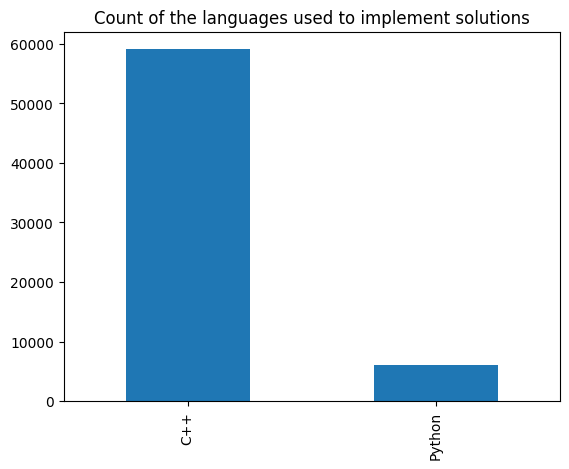
\includegraphics[width=\textwidth]{pics/submissioncount.png}
  \caption{The distribution of the language used for the submissions.}
  \label{fig:dataseteda1}
\end{figure}

\newpage

To fix a bug, the user can do one of the following modifications to the original source code: \textit{replace}, \textit{insert} or \textit{delete}. The distribution of the changes made is similar between the two languages, despite the large difference in the number of submissions Figure \ref{fig:dataseteda2}. For our task, insert and replace changes are the most interesting. Delete is the least interesting because it doesn't require the model to generate any code. And as we found, deletes usually happen in the body of the algorithm to perform debugging.

\begin{figure}[hp!]
\centering
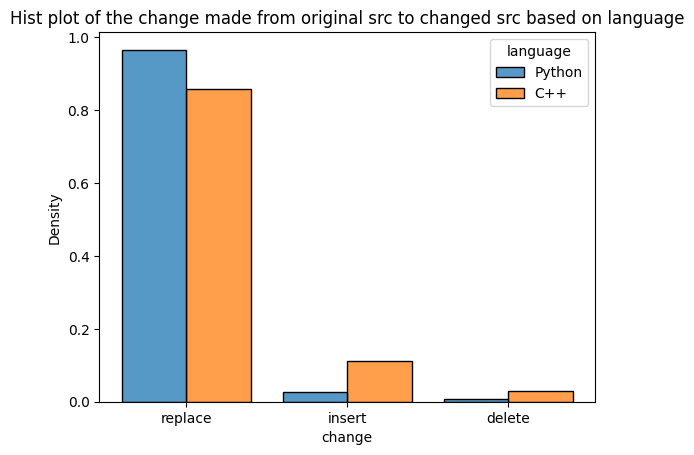
\includegraphics[width=\textwidth]{pics/submissionchange.png}
  \caption{The distribution of the changed made on the buggy source code for each language.}
  \label{fig:dataseteda2}
\end{figure}

\newpage

To check whether the given submission had an input or output bug, we parsed the changes made by the user, and we looked for keywords specific for each language. For example, in Python the function \textit{input} is usually used in the input section of the solution, also \textit{print} is usually used in the output part of the implementation. Similarly, for C++ we looked for \textit{cin} and \textit{scanf}, which are function used to read input, and also for \textit{cout} and \textit{printf}, which are functions used to display the results. We considered the rest of the sections as related to the main algorithm. This is a very naive approach, but it can find the simple sections fairly well, especially in a algorithms solving environment. Most of the bugs are in the algorithm category. We noticed that for Python there are also a lot more input and output bugs compared to C++ Figure \ref{fig:dataseteda3}. This can be due to the fact that Python is a dynamically typed language and it can be easy to make parsing and conversion mistakes on the input or the output.

\begin{figure}[hp!]
\centering
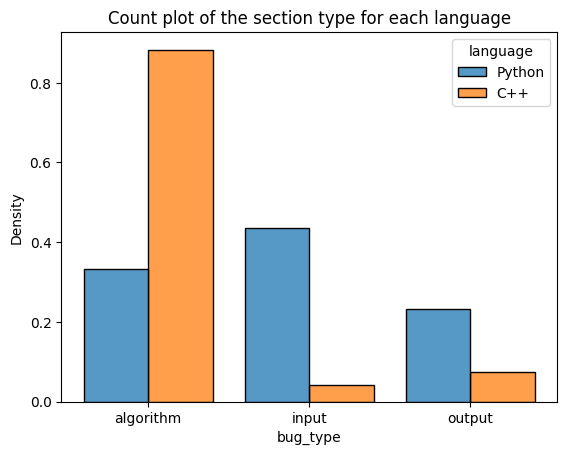
\includegraphics[width=\textwidth]{pics/submissiontype.png}
  \caption{The distribution of the section type of the source code for each language.}
  \label{fig:dataseteda3}
\end{figure}

\newpage

We have also looked at the type of change made for each section type. We found that regardless of the section type, most changes are of type \textit{replace} Figure \ref{fig:dataseteda4}.

\begin{figure}[hp!]
\centering
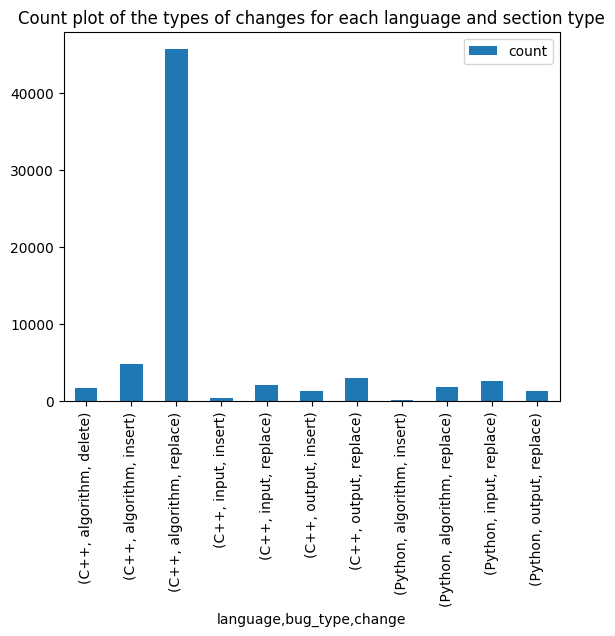
\includegraphics[width=\textwidth]{pics/submissionchangecount.png}
  \caption{The distribution of the change made for each langauge and for each section type.}
  \label{fig:dataseteda4}
\end{figure}

\newpage

Since we removed all the bugs that can be identified using linters and static checks, we are left with the more interesting \textit{Runtime Errors} and \textit{TLEs} and \textit{MLEs} Figure \ref{fig:dataseteda5}. However, most of the bugs are of type \textit{Runtime Error} or \textit{TLE}. We found very few examples of \textit{Out of Memory} bugs.

\begin{figure}[hp!]
\centering
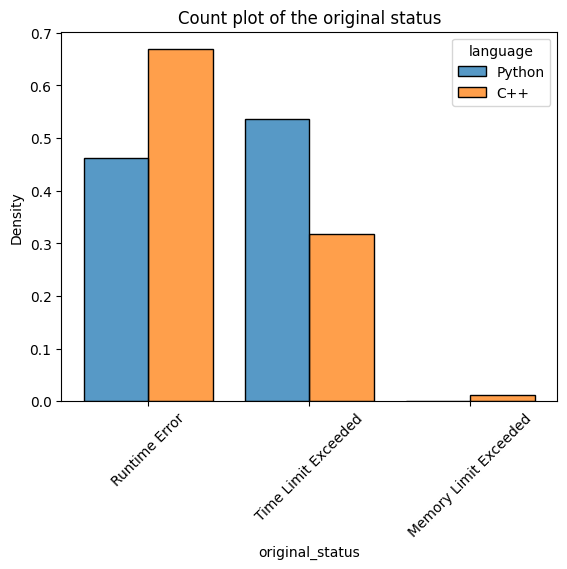
\includegraphics[width=\textwidth]{pics/submissionstatus.png}
  \caption{The distribution of the original status code for the buggy submissions for each language.}
  \label{fig:dataseteda5}
\end{figure}

\newpage

We have executed all buggy examples on the test cases provided in the dataset. However, there are a lot of edge cases that are not covered in the input and output examples. This means that we encounter many zero exit code runs for the buggy examples. This means that we couldn't find the error for such cases, but the source code is still labeled as buggy Figure \ref{fig:dataseteda6}. For C++ most algorithm bugs happen because of TLE and there are also some that fail because of segfault (-11). For C++ input, it is very similar, with more TLE and some segfaults, but this time the distribution between the two errors is more balanced. For C++ output most bugs happen because of TLE. Overall, the most bugs for C++ happen because of TLE. Python is similar, it has mostly TLE bugs. The difference is that for reading input it has some TypeError and ValueError, which can be due to parsing and conversion issues.

\begin{figure}[hp!]
\centering
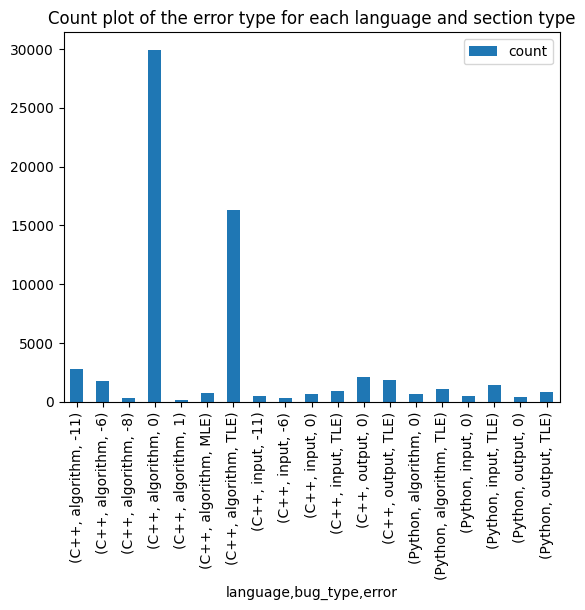
\includegraphics[width=\textwidth]{pics/submissionstatuscode.png}
  \caption{The distribution of the return code of the run on example input for each language and section type.}
  \label{fig:dataseteda6}
\end{figure}

\newpage

We found that most of the bugs happened in the beginning of the file Figure \ref{fig:dataseteda7}, where the figure displays the start line of the chunk that is buggy. For C++ there are some examples where the source code was very long and it exceeds 100 lines, but for Python, most bugs occurred on the first or second line. We can also see that for C++, the starting line of the bug averages around 10. This happens because C++ code usually has more boilerplate code than Python.

\begin{figure}[hp!]
\centering
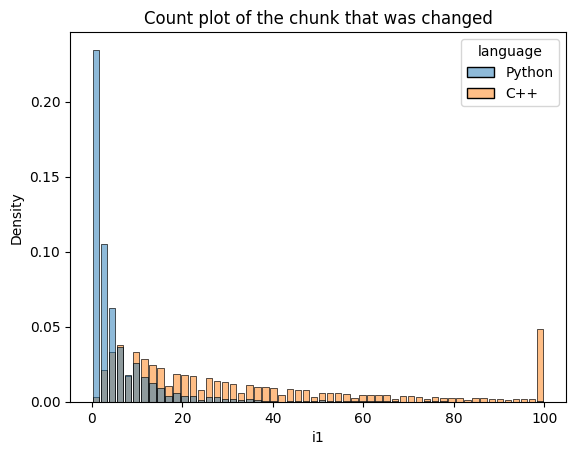
\includegraphics[width=\textwidth]{pics/submissionchunk.png}
  \caption{The distribution of the start line of the chunk that was changed.}
  \label{fig:dataseteda7}
\end{figure}

\newpage

The size of the chunks is similar between the two languages. The most common size for a chunk is one. The size of one represents a single line modification. The number of such chunks is half, which is what we obtained in previous experiments (filtering only one line modifications). There are some zero lines changes, those are the insert changes.  That type of change require code to just be generated and do not require modifications, just insertion.

\begin{figure}[hp!]
\centering
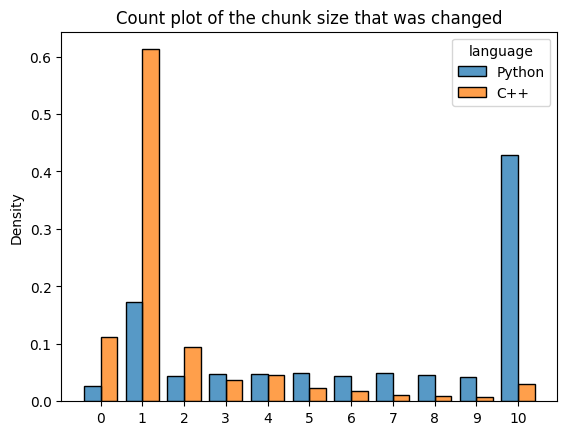
\includegraphics[width=\textwidth]{pics/submissionchunksize.png}
  \caption{The distribution of the size of each chunk that was changed.}
  \label{fig:dataseteda8}
\end{figure}

\begin{table}[htbp]
\centering
\begin{tabular}{|c|c|c|c|c|}
\hline
\multicolumn{1}{|c|}{Language} &  & Bug Type & Error Type & Original Status \\
\hline
C++ & Bug Type & 1.000000 & 0.063548 & 0.070605 \\
\cline{2-5}
& Error Type & 0.063548 & 1.000000 & 0.894415 \\
\cline{2-5}
& Original Status & 0.070605 & 0.894415 & 1.000000 \\
\hline
Python & Bug Type & 1.000000 & 0.131080 & 0.046093 \\
\cline{2-5}
& Error Type & 0.131080 & 1.000000 & 0.495986 \\
\cline{2-5}
& Original Status & 0.046093 & 0.495986 & 1.000000 \\
\hline
\end{tabular}
\caption{Correlation Matrix between the Bug Type, representing the location in code (input, algorithm or output), Error Type, which is the class of the bug, and the Original Status, which is the  value from the original dataset (MLE, TLE or Runtime Error).}
\label{tab:correlation}
\end{table}

We have also split the dataset into three. For the test set, that we used in our evaluation of the models, we have selected the first 30 problems. We choose it like this because the first 30 problems contain 100 Python submissions and that is the threshold that we could use with OpenAI models without any timeouts. Then we have selected the remaining 80\% of the problems for the training set and the last 20\% for the validation set.

\begin{table}[H]\small\linespread{1}
\centering
\caption{Example of buggy source code and the version that was corrected by the user}
\label{tab:experiments7}
\begin{tabular}{p{5cm} p{5cm} p{5cm}}
\textbf{Original Source Code} & \textbf{Changed Source Code} & \textbf{Alternative Change} \\
\hline
\begin{lstlisting}[language=Python]
array = [0, 0, 0, 0]

for i in range(100):
    array[i] = i

print(array)
\end{lstlisting} & \begin{lstlisting}[language=Python]
array = [0] * 100

for i in range(100):
    array[i] = i

print(array)
\end{lstlisting} & \begin{lstlisting}[language=Python]
array = []

for i in range(100):
    array.append(i)

print(array)
\end{lstlisting} \\
\end{tabular}
\end{table}

Usually, a buggy source code will not have a single fix. The modification the user made will also lead to a different instruction, or even multiple instructions, being considered erroneous. Let's take for example the case from the Table \ref{tab:experiments7}, where the bug, an "IndexError", appears in the for loop. The user decided to fix this issue by changing the capacity of the array to fit 100 elements. Now the code works and prints the elements from 0 to 99. When we will compute the code difference we will obtain that the variable initialization of the array caused an "IndexError" bug. This happens because after executing the source code it crashes with that error and the variable initialization is the single change between the two time steps. Intuitively, we will use this example to train the model and it should learn to find similar issues and report them to the user, prompting them to repair the code.

\begin{table}[H]\small\linespread{1}
\centering
\caption{Example of a correct source code and the steps taken from the original source code}
\label{tab:experiments8}
\begin{tabular}{p{5cm} p{5cm} p{5cm}}
\textbf{Alternative Change - step 1} & \textbf{Alternative Change - step 2} & \textbf{Alternative Change} \\
\hline
\begin{lstlisting}[language=Python]
array = []

for i in range(100):
    array[i] = i

print(array)
\end{lstlisting} & \begin{lstlisting}[language=Python]
array = [0, 0, 0, 0]

for i in range(100):
    array.append(i)

print(array)
\end{lstlisting} & \begin{lstlisting}[language=Python]
array = []

for i in range(100):
    array.append(i)

print(array)
\end{lstlisting} \\
\end{tabular}
\end{table}

The user can make some other modifications, such as the Alternative Change from the Table \ref{tab:experiments7}. This produces the same output as the previous fix, but has some other side effects on how the model will work. Since there are two modifications in the source code, we have to check what error each of them fixes. In Table \ref{tab:experiments8} are presented the two intermediate steps that are checked, the first step will modify only the array initialization, and the second step will modify only the body of the for loop. As expected, the first step will fail with an "IndexError", since the array has zero capacity. On the other hand, the second step will work, in the sense that it will not throw any errors, but it will not output the correct result. Interestingly enough, the bug that was found in the source code was still the initialization of the array, with the same category, but with a different fix from the other attempt.

\subsection{Experiment Setup}

\subsubsection{Metrics}

\textbf{Exact Match}. For this exepriment we have used the \textit{Exact Match} metric, which computes the accuracy by comparing the generated code with the accepted code

\textbf{Pass@K}. We have also used \textit{Pass@K}, which runs the generated code against a set of test cases to compute the accuracy. The K parameter refers to the number of examples that the model generated. The prediction is considered correct if any prediction passes the tests.

\subsubsection{Models}

\textbf{Codex}. As mentioned, Codex is a large language model used for generating source code in many different programming languages. However, it can also generate comments and natural language at some extent in a question and answering manner. For the first experiment we wanted to check how well is Codex going to perform on repairing identified mistakes in source code. This means that we are going to mark the bug in the source code using a \textit{fixme} comment and let the model predict a solution for that bug. 

In the experimental setup we have used the default parameters of the Codex model: with \textit{temperature} of 0.5 \textit{max\_tokens} of 256 and \textit{top\_p} of 1. We ran the experiment on a sample of 200 submissions, with 100 C++ submissions and 100 Python submissions. We performed the experiment 5 times and chose the best results. The reasoning for using only 100 submissions per language is that the API calls need to be delayed by $\sim$15 seconds to not reach the rate limit and each experiment run can take up to 5 hours.

\textbf{ChatGPT}. ChatGPT does not have a free public API yet so the only way to evaluate it is to manually test each submission. We have used the same prompting as in the Codex evaluation.

\textbf{CodeGen2}. For the CodeGen2 model we have used the 1B parameters model \footnote{https://huggingface.co/Salesforce/codegen2-1B}. We have tested the infilling capabilities of the model on our bug examples. For this task we have made use of three tokens introduced in the paper, $<mask_N>$, $<sep>$ and $<eom>$. We have built the prompt using a formatting function such that we mask the bug and ask the model to predict a replacement. Thus, the prompt will look like \textit{prefix}$<mask_1>$\textit{suffix}$<|endoftext|>$$<sep>$$<mask_1>$. This will prompt the model to generate a completion for the $mask_1$ token. To have a similar approach to the training method described in the paper we have stopped the generation when the model predicted the $<eom>$ (end of message) token. For example the output of the pipeline will be \textit{prefix}$<mask_1>$\textit{suffix}$<|endoftext|>$$<sep>$$<mask_1>$\textit{prediction}$<eom>$. We have also set a maximum number of tokens to 512, since the problems in the BugNet dataset are rather short. Finally, we have generated 2 examples for each problem and tested using the discussed metrics.

The largest model from CodeGen2 has 16B parameters. However, due to GPU limitations we were not able to test it. This proved to be a huge factor because the 1B parameter was able to fix only one Python example. However, we have noticed that most of the completions made by CodeGen2 were syntactically correct and the code would compile.

\textbf{OpenAssistant}. OpenAssistant does not provide API access yet so we are limited to manually testing the problems. For this experiment we have used the k50 preset, with a \textit{temperature} of 0.75, \textit{max\_new\_tokens} of 1024 and \textit{top\_p} or 0.95.

\subsubsection{Overview}

The main challenge for this experiment comes from prompt engineering, because we need to express well enough the task that the model needs to perform. The other problem comes from the model generating some correct responses but it uses human language to describe what to do, even if it includes code. We have iterated in the Codex playground for different prompts \footnote{https://beta.openai.com/playground}. 

We have tried to just add a comment with the text \textit{fixme} at the end of the line that contained a bug, but this did not work. Then we tried to add a \textit{Solution:} comment at the end to make the model generate some source code, however this led to very bad performance, Codex being able to fix only one bug from the 200 tested. 

One of the best prompt was to use a Q\&A style prompt. We have still used the \textit{fixme} comment but also added at the end two line comments one with the question \textit{Q: Propose a fix for the buggy line of code} and another one with a simple \textit{A:} that should be filled by the AI. This showed some decent qualitative results, but can be hard to accurately predict a score, since it would sometimes use more than just the fix to describe the solution. Adding extra requirements to the "Q" part of the prompt can increase the prediction accuracy. For example modifying the prompt to \textit{Q: Propose a fix for the buggy line of code, using a single line of Python code}, doubled the accuracy of the predictions for the Python language. Of course the name of the language should be the same as the one used in the implementation.

\subsection{Qualitative Evaluation}

\subsubsection{Examples of prompts used and Codex results}

For the first prompt, with just the \textit{fixme} comment, there were a lot of empty responses from the model, especially on the C++ source code.

\begin{lstlisting}[language=C++]
#include <stdio.h>
int main(void) {
  int a = 0, b = 0, c = 0, n, t;
  while (scanf("%d", &n)) { // fixme
    if (n > a)
      t = n, n = a, a = t;
    if (n > b)
      t = n, n = b, b = t;
    if (n > c)
      c = n;
  }
  printf("%d\n%d\n%d\n", a, b, c);
  return 0;
}
\end{lstlisting}

For the \textit{Solution} comment at the end of the prompt the model would predict source code most of the times, but as we saw in the results, the accuracy was not that good.

\begin{lstlisting}[language=C++]
#include <stdio.h>
int main(void) {
  int a = 0, b = 0, c = 0, n, t;
  while (scanf("%d", &n)) { // Fixme
    if (n > a)
      t = n, n = a, a = t;
    if (n > b)
      t = n, n = b, b = t;
    if (n > c)
      c = n;
  }
  printf("%d\n%d\n%d\n", a, b, c);
  return 0;
}
// Solution:
\end{lstlisting}

For this particular code the Codex model predicted:

\begin{lstlisting}[language=C++]
#include <stdio.h>
int main(void) {
  int a = 0, b = 0, c = 0, n, t;
  while (scanf("%d", &n) != EOF) {
    if (n > a)
      t = n, n = a, a = t;
    if (n > b)
      t = n, n = b, b = t;
    if (n > c)
      c = n;
  }
  printf("%d\n%d\n%d\n", a, b, c);
  return 0;
}
\end{lstlisting}

The resulted source code still compiles, and also fixes the bug. However, this is not the solution that the user found, so it was marked as incorrect, even though it is a valid submission.

For the last type of prompt the model usually generates a single line of code, or a couple lines of comments mixed with code. And this type of prompt seems to provide the best quality answers.

\begin{lstlisting}[language=C++]
#include <stdio.h>
int main(void) {
  int a = 0, b = 0, c = 0, n, t;
  while (scanf("%d", &n)) { // Fixme
    if (n > a)
      t = n, n = a, a = t;
    if (n > b)
      t = n, n = b, b = t;
    if (n > c)
      c = n;
  }
  printf("%d\n%d\n%d\n", a, b, c);
  return 0;
}
// Q: Propose a fix for the buggy line of code
// A:
\end{lstlisting}

For this example the Codex model predicted 

\begin{lstlisting}[language=C++]
while (scanf("%d", &n) != EOF) {
\end{lstlisting}

which is just the replacement for the buggy source code. However, we still face the same issue, that the code is functional, but this cannot be checked due to limited test cases and the fact that the user changed the buggy code in a different manner:

\begin{lstlisting}[language=C++]
while (scanf("%d", &n) > 0) {
\end{lstlisting}

In theory the \textit{scanf} function can return either \textit{EOF} if the end of input is reached, \textit{0} if there was an error on reading the input and in case of success it returns the number of correctly parsed arguments. So arguably, the solution that Codex found, although would work on the problem and probably on all test cases, is less correct than the solution that the user found. This is because it does not take into account the case where the input is not a number. 

Some of the responses of the Codex model:

\begin{enumerate}
\item \textit{Delete the line of code and add vector\textless{int}\textgreater mountain(10)}
\item \textit{printf("\%d$\backslash{n}$", array[9-i]);}
\item \textit{Change the input format to \&height[i]}
\item \textit{remove the while loop and make it a for loop}
\end{enumerate}

These examples show some of different types of results that the model can predict, ranging from just simple code to natural language instructions. The natural language instructions could be very interesting to be used in an application where based on the code that you have wrote so far in a coding challenge you can ask an AI for hints on how to fix a part of your code that makes you stuck. This lead us to investigate a much better language model, that can provide us with any of the answers by instructing it how much details to reveal, which is ChatGPT.

\subsubsection{ChatGPT results}

We were able to use ChatGPT to not only find the solution, but to also identify the bug category. For example, when fed the previously discussed code sample, it named the title of the conversation \textit{Fixing infinite loop in C} and it managed to answer with the following helpful message:

\textit{One possible fix for the buggy line of code is to replace "while (scanf("\%d", \&n))" with "while (scanf("\%d", \&n) != EOF)" to correctly detect the end of input. This will ensure that the loop only runs while there are still input values to read, and will prevent the program from running indefinitely.}

To continue the idea of providing hints to help with coding challenges we can use a prompt similar to the Q\&A type, but replace the question with the template: "\textit{Q: Propose a hint that can help me fix the bug}". Again as an example, we can use the same source code as before:

\begin{lstlisting}[language=C++]
#include <stdio.h>
int main(void) {
  int a = 0, b = 0, c = 0, n, t;
  while (scanf("%d", &n)) {
    if (n > a)
      t = n, n = a, a = t;
    if (n > b)
      t = n, n = b, b = t;
    if (n > c)
      c = n;
  }
  printf("%d\n%d\n%d\n", a, b, c);
  return 0;
}
// Q: Propose a hint that can help me fix the bug
// A:
\end{lstlisting}

On this prompt, ChatGPT provided the following answers which describe the right action that the user has to perform:

\textit{Add a condition to the while loop to exit when the input is invalid (such as reaching the end of the file) or when the desired number of inputs have been read.}

or

\textit{Check if the input scanf is reaching the end of the file or if there is an error in input by using the return value of scanf and breaking out of the loop when necessary.}

which is indeed the right action that the user has to perform. Notice that ChatGPT does not require any annotations in the code and it can even detect the bug by itself more often than Codex does. For example, if we provide the same input to the Codex model we would get the following answer:

\textit{Make sure to check if the user input is still within the range of the variables after swapping the values.}

which does not make any sense. But if we keep the \textit{fixme} comment we just get the direct solution:

 \textit{Replace the while loop condition with scanf("\%d", \&n) != EOF}

 which is correct, but not what we asked the model to do.

 In one recent study \cite{https://doi.org/10.48550/arxiv.2301.08653}, that uses the QuixBugs \cite{10.1145/3135932.3135941} benchmark, it was reported that ChatGPT was able to fix 19 out of 40 bugs. This has a higher accuracy than we obtained using CodeT5, but the programming language differs. Also the problems given in QuixBugs are mostly popular algorithms, while in CodeNet we have many programming challenges.

\subsection{Quantitative Evaluation}

The results for the best performing prompt are presented in Table \ref{tab:codex1}. The prompt that we used was a Q\&A style prompt where the initial text is the buggy source code, with the \textit{Fixme} comment on the line that includes the bug, and the \textit{Q: Propose a fix for the buggy line of code, using a single line of Python code} and \textit{A:} extra comments that tell Codex what the task is about. In the results we can see that Codex can fix 10\% of the bugs given in Python source code, but it is unable to solve hardly any bugs on the C++ subset. We can notice that the accuracy of the Codex model is very bad on our dataset. The first issue comes from comparing the suggestion of the model with the ground truth for an exact match. This is a problem because the ground truth solution might not be the only possible fix for the given bug. We can solve this problem by using the test cases to decide if a problem was fixed. This way we wouldn't even need the ground truth solutions. However, the dataset does not include all the test cases. And the test cases that are available in the original dataset are not enough to precisely determine which sources are buggy in the first place. There are many submissions labeled as not accepted passing the given tests. The other issue comes from the Codex model sometimes outputting descriptions with the steps that you need to make to fix the problem, without always including the source code.

\begin{table}[H]\small\linespread{1}
\centering
\caption{Quantitative results of the Codex Bug Repair Experiment using the best Q\&A prompt using exact match accuracy between the generated code and the changed code}
\label{tab:codex1}
\begin{tabular}{p{4cm} l >{\raggedright\arraybackslash}p{2cm} >{\raggedright\arraybackslash}p{2cm} >{\raggedright\arraybackslash}p{2cm} >{\raggedright\arraybackslash}p{2cm}}
\textbf{Language} & \textbf{Accuracy} \\
\hline
C++                                 & 0.002 \\
\hline
Python                              & 0.108 \\
\end{tabular}
\end{table}

The qualitative results look much better, despite the low accuracy of the Codex model. We have built a demo plugin for neovim to access the Codex API and predict hints for buggy source code \footnote{https://github.com/alexjercan/codehint}. It can be quite difficult to quantify the performance of such tool, but visually it can give correct hints, in some cases.

To look further into the big difference between the qualitative and quantitative results we have also computed the accuracy in terms of execution. This means that we took the code that was generated by the Codex API and we have tested it on the test cases from the dataset. Considering the execution accuracy notated as pass@1 we have observed that there are more fixes that we originally found using exact match comparison. 

\begin{table}[H]\small\linespread{1}
\centering
\caption{Quantitative results of the Codex Bug Repair Experiment using the best Q\&A prompt using pass@1 accuracy for the generated code on the test cases in the dataset}
\label{tab:codex2}
\begin{tabular}{p{4cm} l >{\raggedright\arraybackslash}p{2cm} >{\raggedright\arraybackslash}p{2cm} >{\raggedright\arraybackslash}p{2cm} >{\raggedright\arraybackslash}p{2cm}}
\textbf{Language} & \textbf{Accuracy} \\
\hline
C++                                 & 0.03 \\
\hline
Python                              & 0.43 \\
\end{tabular}
\end{table}

In Table \ref{tab:codex2} we have shown the results when using execute accuracy for the generated code. This aligns more with the quality of the responses that we have visualized. The execution accuracy for Python matches with the code generation accuracy that was presented in related work. 

We have also grouped the evaluation data into \textit{input}, \textit{output} and \textit{algorithm} categories and checked the capabilities of the Codex model to fix these types of bugs. The \textit{input} category includes the source code files that contain a bug (a change between the original source code and the accepted source code) that includes the reading functions specific to the languages used. The \textit{output} section is similar containing bugs that use printing functions. The remaining bugs are categorized as \textit{algorithms} bugs. We have found that the dataset contains more input bugs than the other two categories. We found that Codex does best on \textit{output} bugs \ref{tab:codex3}, however we had the fewest examples in that category.

\begin{table}[H]\small\linespread{1}
\centering
\caption{Quantitative results of the Codex Bug Repair Experiment using the best Q\&A prompt using pass@1 accuracy for the generated code on the test cases in the dataset for the Python language. This represents an expansion of the previous results, but split into the three categories.}
\label{tab:codex3}
\begin{tabular}{p{4cm} l >{\raggedright\arraybackslash}p{2cm} >{\raggedright\arraybackslash}p{2cm} >{\raggedright\arraybackslash}p{2cm} >{\raggedright\arraybackslash}p{2cm}}
\textbf{Category} & \textbf{Fixed} & \textbf{Total} & \textbf{Accuracy}  \\
\hline
algorithm	      & 8              & 16             & 0.50 \\
\hline
input	          & 28             & 72             & 0.38 \\
\hline
output	          & 7              & 12             & 0.58 \\
\hline
\end{tabular}
\end{table}

\section{AoC Eval}

\subsection{Data Exploration}

In this section we will discuss the particularities of the AoC Eval dataset, and also what we have learned by using a smaller evaluation set on large language models. The dataset that we used in this experiment contains 15 submissions for a range of easy to intermediate problems that fail on the test cases provided by the competition.

The AoC dataset contains mostly replacement and some insertions. In most cases of programming a deletion would occur because the user forgot to delete a debugging print statement, which is not hard to repair manually. Insertions would happen when the user forgets to handle an edge case, which can be interesting to identify using machine learning. Such edge cases can be inferred from the constraints in the problem statement, but not only. In problems from advent of code, most edge cases tend to arise from the formatting of the input and thus the data structure selection of the user. Most of the bugs however will be of type replace. This means that the user changed something in the buggy code to make it work.

\begin{figure}[hp!]
\centering
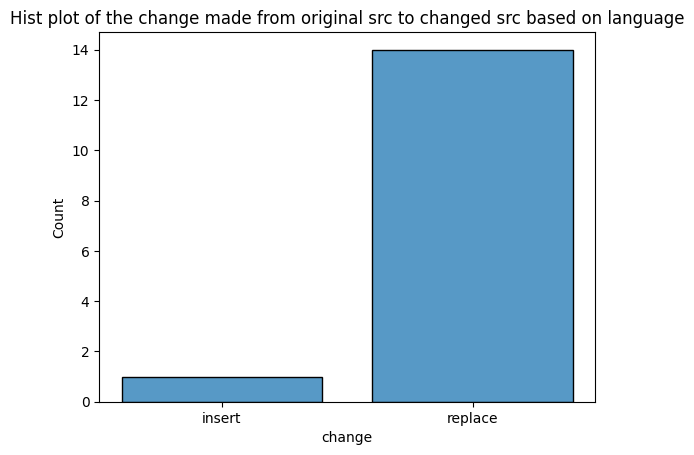
\includegraphics[width=\textwidth]{pics/aoc_submissionchange.png}
  \caption{The distribution of the change made in the submissions.}
  \label{fig:aoceda1}
\end{figure}

In Figure \ref{fig:aoceda1} we show the distribution of change types in our dataset. The reasoning that most of the changes are replace is to match the distribution of real life cases.

Bugs can happen anywhere in the file, but we have found (especially in BugNet) that in many examples the changed line was in the first four of five lines of code. This usually tends to happen because the problems are very simple. Another possibility for the change to start in the beginning of the file is if the user has changed the entire file (or a big portion of it). For the cases where this happens we have found a high correlation between the starting line of the chunk and the size of the chunk. Thus, a single chunk difference might not always be the best approach, especially when the difference is the entire file. One solution to this issue can be filtering by the size of the chunk. The problem can be stated as finding the value for the maximum number of lines in a code diff such that by adding that bug example it would improve the quality of the dataset.

\begin{figure}[hp!]
\centering
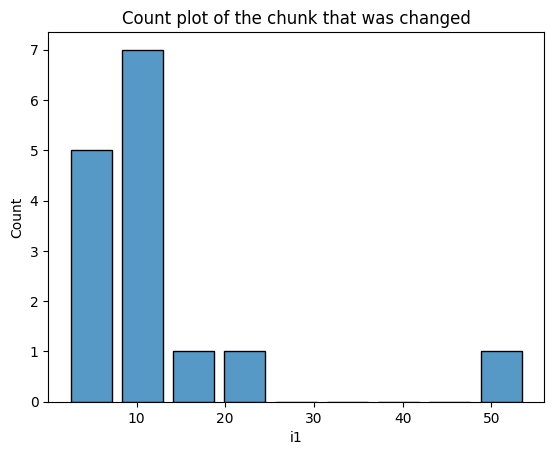
\includegraphics[width=\textwidth]{pics/aoc_submissionchunk.png}
  \caption{The distribution of the starting line of the chunk that was changed in the submissions.}
  \label{fig:aoceda2}
\end{figure}

In the case of really simple problems, there were many changes in parsing of the input. In the AoC Eval dataset we have tried to focus only on bugs that are not related to parsing the input or showing the output, but more on solving the problem. We have also tried to work on the problem of having whole file difference between two submissions, by including only small changes in the code to make it work as seen in Figure \ref{fig:aoceda3}. Thus, we have almost 90\% of the submissions with a number of lines changed of less than five.

\begin{figure}[hp!]
\centering
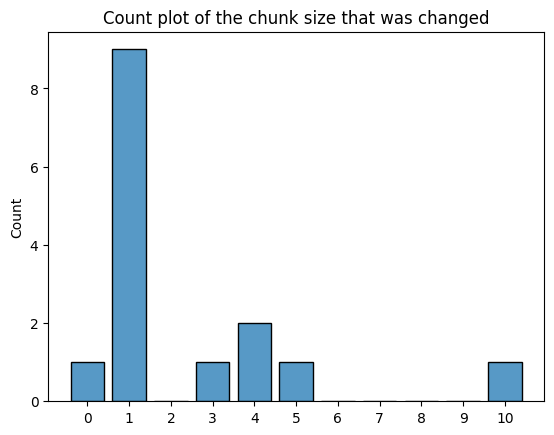
\includegraphics[width=\textwidth]{pics/aoc_submissionchunksize.png}
  \caption{The distribution of the starting line of the chunk that was changed in the submissions.}
  \label{fig:aoceda3}
\end{figure}

In the case of BugNet we have thought that the size of the chunk (block of code that was changed) would play the biggest factor in making the task of repair easier. However, when testing with the AoC Eval dataset, we have noticed that large language models, like ChatGPT and OpenAssistant, have struggled to find repairs for even one line changes. In fact the most important factor was the using of the problem statement in the input prompt. This made the difference between providing the user with a meaningful hint for solution for the bug at hand or not.

\subsection{Experiment Setup}

\subsubsection{Setup}

We have replicated the experimental setup that we did for the BugNet dataset. Thus we have used the ChatGPT\footnote{ChatGPT May 24 version https://help.openai.com/en/articles/6825453-chatgpt-release-notes}, OpenAssistant and CodeGen2 models with the same prompt and parameters as described in the BugNet experiments section. We were not able to also use Codex because it was deprecated since we did our last experiment. For a second part of our experiment, we have also worked with improved prompting strategies, discussed in related work.

\subsubsection{Overview}

The tasks that we tried in this experiments are code completion and generating natural language hints for bugs in code. Code completion results can be quantified using the described metrics, however we cannot easily measure the usefulness of hints generated by AI. Thus, we have also tried to run the experiment of generating hints on a group of people by asking them prompts and getting responses in a similar way that the interaction with ChatGPT works. This way we can compare the responses of language models to the responses of our human testers.

To better understand the task of hint generation from buggy code we have tried a few methods.

\textbf{Blind hint generation}. Blind hint generation is a task where the user provides in the prompt only the source code with no additional information. We found that both humans and AI can struggle to find the correct solution. The difference that we have noticed in the way that humans tend to respond to suggesting hints is that they tunnel vision on a specific portion of the code and the quality of the responses is a guessing game of whether they have found the problem from the first try or not. On the other hand, AI is capable of suggesting many more hints, for almost all blocks of execution, in the end also resorting to a guessing game, this time asking the question of which hint to investigate first. To make the comparison fair between the two categories we will consider a similar metric to Pass@K, where K will represent the number of hints allowed to be generated. This way, a Pass@1 would make a fair comparison between the human responses and the AI responses. We will refer to this metric as Hint@K, to not create confusion with the code completion task.

\textbf{Hint generation with problem statement}. The second method that we tried, which improved the evaluation dramatically, is providing the testers with the problem statement. We have observed that humans were able to give useful hints for almost all the problems in the evaluation set after being faced with the problem statement. ChatGPT was also able to find the bugs in the code when prompted with both the code and the problem statement. However we have found an interesting situation where ChatGPT was not able to provide the correct hint for a problem where human testers were able to find the problem without the problem statement, which we will discuss in the results section.

\textbf{Blind Hint generation with Chain of Thought}. We have tried to simulate the Chain of Thought (CoT) mechanism by asking the language model to first make a step by step explanation of the source code, and only after to give the list of potential bugs. This has proved to get much better results on the AoC evaluation set.

\subsection{Results}

Since we have manually reviewed all the problem solutions, we knew that the bugs are really hard to find by looking only at the source code regardless of the prompt. As long as we didn't hint towards where the issue was, the models, but also human testers, were not able to find most of the bugs. However, we have still tried to improve the prompts that used only source as much as possible. For example, using a really straight forward prompt like "What is a potential problem with the following code?" would result most of the times in responses that target formatting, variable naming conventions, documentation and unit testing (or lack thereof). By changing this prompt to use a plural form, "What are some potential problems with the following code?" we were able to generate a list of potential hints. As one might guess, the issue of being told that the problem is related to documentation or testing still remained. This happened because the given prompt was too generic and probably very similar to training data that included such type of interactions between users. For ChatGPT we do not know exactly where the training data comes from, but we can make a guess that it includes a large portion of StackOverflow\footnote{https://stackoverflow.com/}. In the case of GPT2 we know that StackOverflow made up 0.1\% of the training data, and GitHub made up 1\% of the training data\footnote{https://github.com/openai/gpt-2/blob/master/domains.txt}. On the other hand, OpenAssistant has the training data publicly available, and consists mainly of human generated inputs made specifically for training the model. In both cases, there can be many examples where users asked for opinions on source code that is part of a project or a module, so hints about formatting, conventions and documentation make sense. But in our case we need more specific hints, since we only want to use the code once for a coding submission.

One prompt that generated some of the desired results only on source code was "You are an expert bug finder for \textless{LANGUAGE}\textgreater{ }code submissions to algorithm problems.  Give me a list of potential problems that I can have in this code. Focus only on bugs that are relevant to solving the problem. Disregard maintainability or readability concerns. \textless{CODE}\textgreater". Using this prompt we have managed to get more specific answers from both  OpenAssistant and ChatGPT. By more specific answers we mean hints that actually reference values and variables in code. As seen in Table \ref{tab:aoc1}, both the human testers and the language models performed poorly when given only the source code. We have observed that we got much better hints when using the problem statement in the prompt as well.

\begin{table}[H]\small\linespread{1}
\centering
\caption{Quantitative results of the AoC Bug Hint Experiment. We have found that human evaluators had the best results. In total we had 15 prompts. ChatGPT managed to provide 13/15 useful hints when given the problem statement and allowed to generate multiple predictions.}
\label{tab:aoc1}
\begin{tabular}{p{4cm} l >{\raggedright\arraybackslash}p{2cm} >{\raggedright\arraybackslash}p{2cm} >{\raggedright\arraybackslash}p{2cm} >{\raggedright\arraybackslash}p{2cm}}
\textbf{Group}    & \textbf{Blind Fixes} & \textbf{With Problem Statement} & \textbf{CoT Blind Fixes}  \\
\hline
ChatGpt@1         & 1                    & 1                               & 5 \\
\hline
ChatGpt@5         & 4                    & 13                              & 8 \\
\hline
OpenAssistant@1   & 0                    & 1                               & - \\
\hline
OpenAssistant@5   & 2                    & 1                               & - \\
\hline
Human Evaluators  & 3                    & 14                              & - \\
\hline
\end{tabular}
\end{table}

While using the problem statement in the prompt, we have also found that the quality of the question is not as important as it was before. For example, having a prompt like "\textless{STATEMENT}\textgreater \textless{CODE}\textgreater What is the bug in the code?" already had better results than the best prompt that we engineered using only source code. In the end we have learned that both humans and language models benefit a lot from the added context of the problem statement.

While including the problem statement in the given prompt has seen huge improvements in finding the bug in the code, prompting the LLM to also predict the explanation for each instruction in the code had similar effects. By using a prompt of the form "Provide a step by step analysis of the code. Based on the analysis create a short summary with the top most probable bugs that can happen in the given code.  \textless{CODE}\textgreater" we have seen much better responses from ChatGPT. However, we have also noticed mistakes in the chain of thought. We have found that for some buggy instructions, the model would predict what the correct version of the instruction should be doing, instead of what is actually happening.

In an attempt to help the LLM to give better predictions, we needed to make it evaluate each step. For example we can try to make it generate an example of the input and the output and to try to evaluate the step, in a similar way to the ToT implementation "Provide a step by step analysis of the source code, at each step show an example using the instruction and answer the question \textless{Is the prediction correct?}\textgreater.", then would follow the rest of the prompt. We have found that the step by step analysis with examples was really valuable in identifying bugs for a human. 

An improvement of the current prompt was to ask the LLM to give an example of input and output for the predicted bug and also reference the step that caused the prediction. This means that we changed the second part of the prompt to "Based on the analysis provide a list of the most probable bugs. For each bug give a short explanation with input and output examples and relate it to the corresponding step from the analysis.". With this strategy we have managed to find 8/15 bugs compared to only 4 with the IO prompt. However, we are still facing the issue that the LLM is not capable of predicting good enough hints even with clear examples that showcased the bug.

\subsubsection{Human Only Fixes}

We have found one case in which the human evaluators were able to identify an issue in the code, but the language models like ChatGPT and OpenAssistant were not able to identify even after being provided with the problem statement.

For example in the given code the programmer was trying to solve a rock paper scissors game, where for player 1 the actions are labeled with ABC and for the second player they are labeled with XYZ.

\begin{lstlisting}[language=Python]
def solve(test: str) -> str:
    points = {"X": 1, "Y": 2, "Z": 3}
    beats = {"X": "C", "Y": "A", "Z": "B"}

    lines = test.strip().splitlines(keepends=False)

    score = 0
    for line in lines:
        fst, snd = line.split(" ")

        if fst == beats[snd]:
            score += 6
        elif fst == snd:
            score += 3

        score += points[snd]

    return str(score)
\end{lstlisting}

The problem here lies in the fact that the coder made a wrong check in the \textit{elif} condition.

\begin{lstlisting}[language=Python]
if fst == beats[snd]:
    score += 6
elif fst == snd:
    score += 3
\end{lstlisting}

Human evaluators were able to identify the problem, and for example gave hints such as "fst == snd will never be true", which is correct, the coder should have done instead \textit{fst == mapping[snd]}. ChatGPT was trying to give hints focused on safety, such as "If the input contains a character that is not a key in these dictionaries, a KeyError will be raised.", and it was a similar case with OpenAssistant. Then even with the problem statement, the suggestions were not improving.

The issue might be caused by the really complicated statement of the problem, and the use of unintuitive variable naming. However, this is to be expected from a coding challenge.

\subsubsection{ChatGPT Blind Fixes}

We have also found cases where the language models were able to identify bugs that humans were not able to find. Albeit humans testers were still able to figure out the issue when provided with the problem statement and more time.

For example in the given code, the user wants to find the maximum sum in a list of list of numbers.

\begin{lstlisting}[language=Python]
def solve(test: str) -> str:
    chunks = test.strip().split("\n\n")
    current = 0
    maximum = 0

    for chunk in chunks:
        numbers = map(int, chunk.splitlines())
        for number in numbers:
            current += number

        if current > maximum:
            maximum = current

    return str(maximum)
\end{lstlisting}

Without the problem statement, the human evaluators thought the the code is trying to find the maximum number for the lists. In this case the variable name \textit{maximum} caused the confusion. Thus, the hint they tried to provide was that we should not use a \textit{current} variable and just check against the number to find the maximum. The main difficulty came from the fact that it is more common to be tasked with finding the maximum from a list. And as we noticed in this experiment humans tend to tunnel vision on only one aspect, in this case the \textit{maximum} variable name, which was more familiar and disregarding things that are harder to understand on a first glance, such as splitting on double new lines and maps.

On the other hand, ChatGPT managed to find the real issue and suggested "The current variable is not reset to 0 at the start of each chunk iteration." However, OpenAssistant was not able to predict a useful hint even with the problem statement.

\subsubsection{General Blind Fixes}

There is also one case were both the human evaluators and ChatGPT were able to identify a problem without a need for the problem statement. In this case the issue was with the typing of a variable, so the problem statement had less relevancy to the issue.

\begin{lstlisting}[language=Python]
import string


def solve(test: str) -> str:
    priorities = dict(
        enumerate(
            string.ascii_lowercase + string.ascii_uppercase, 
            start=1,
        )
    )

    lines = test.strip().splitlines(keepends=False)

    priority = 0
    for line in lines:
        midpoint = len(line) // 2
        part1, part2 = set(line[:midpoint]), set(line[midpoint:])

        common = "".join(part1.intersection(part2))

        priority += priorities.get(common, 0)

    return str(priority)
\end{lstlisting}

In this submission the coder tried to create a priorities dictionay that is used to compute the priorities of some strings. Since the humans were able to infer that the priority should be a number, they quickly realised that the priorities dictionary is not built correctly. In the current implmentation the programmer create a dictionary from a number to a character, but we would need it to be the other way around.

This time both the human evaluators and ChatGPT were able to give useful hints. However, both groups have predicted an extra hint for a potential bug in how the common variable is is used with the priorities dictionary. Both humans and ChatGPT predicted that we might have multiple common characters between two parts, and the \textit{get} method would fail. When faced with the problem statement, which had a restriction that claimed that the size of \textit{common} will always be 1, both groups changed their predictions to include only the hint about how the priorities are created. Thus, both groups realized that the check for \textit{common} to be of length 1 would be redundant.

\subsubsection{With Problem Statement}

For the next problem, neither the human group or the language models were not able to find a hint without the problem statement. In this problem, the user is tasked with traversing a file system and calculating the total size of items with size smaller than a threshold.

\begin{lstlisting}[language=Python]
def calculate_directory_size(directory, cwd, sizes):
    size = 0
    for name, content in directory.items():
        current_name = cwd + name + "/"

        if isinstance(content, int):
            size += content
        else:
            size += calculate_directory_size(
                content, current_name, sizes
            )

        sizes[current_name] = size

    return size


def solve(test: str) -> str:
    ...

    sizes = {}
    for _, content in filesystem.items():
        calculate_directory_size(content, "/", sizes)

    total = 0
    for _, size in sizes.items():
        if size <= 100000:
            total += size

    return str(total)
\end{lstlisting}

When provided with the problem statement, OpenAssistant managed to find the issue and predicted "There could be an issue where the calculate\_directory\_size function does not properly handle nested directories when calculating the total size. This could lead to an incorrect total size calculation."

Here the problem was that the line \textit{sizes[current\_name] = size} should be replaced with \textit{sizes[cwd] = size} in computing the size of the current directory.

The code snippet does not include the parsing of the input, which would make the code harder to understand. By omitting that section of the code, the human evaluators were able to find the issue, just from the code. By reducing the size of the code, we also get better results from language models from the source code only prompts.

In this case, the problem statement would only help with the calculation of the total variable. But we would expect that by reading the problem statement one might be able to validate what is correct or not in the implementation and then focus on the parts that might not be very clear.

\subsubsection{Chain of Thought}

For this example, ChatGPT was able to find the fix only when given the problem statement. In this problem we wanted to showcase how the LLM will predict that the source code is doing what it is intended to do, but it is actually wrong.

\begin{lstlisting}[language=Python]
import string


def solve(test: str) -> str:
    priorities = {
        c: v
        for v, c in enumerate(
            string.ascii_lowercase + string.ascii_uppercase, 
            start=1
        )
    }

    lines = test.strip().splitlines(keepends=False)

    priority = 0
    for i in range(0, len(lines), 3):
        common = "".join(
            set(lines[i]) & set(lines[1]) & set(lines[2])
        )

        priority += priorities.get(common, 0)

    return str(priority)
\end{lstlisting}

In this problem the user is supposed to compute the intersection of three consecutive lines. However, the coder made a typo and instead of using $i$, $i+1$ and $i+2$, they used $i$, $1$ and $2$. 

The prediction of ChatGPT had the correct intention "The code enters a loop that iterates over the range from 0 to the length of lines with a step of 3. This means it will process three lines at a time.". Since this is a very common construct used in many programs, the LLM did not manage to reason that the next line contained a mistake, and assumed that it will be correct as well "Inside the loop, the common variable is assigned the intersection of characters present in the first line, second line, and third line. The set function is used to convert each line into a set of characters, and the \& operator performs the intersection operation." Finally the model predicted "Based on the analysis, the code seems to be functioning correctly.". If we ask ChatGPT to evaluate it's prediction compared to the code it manages to figure out the mistake. Thus it would probably make sense to have a database of possible hints, or generate hints using a model, and then predict the best match using another model, by evaluating each combination.

\chapter{Conclusion}

We presented the problem of bug detection and repair with some of the most recent approaches that attempt solving it. We have discussed the process of creating a dataset with labeled instructions from existing code submissions to online coding competitions. As an example we have created BugNet, which is a dataset that can be used to finetune transformer based models to repair code. We have also introduced AocEval, which is a benchmark dataset for the task of bug detection and repair. We have showed how to identify buggy code with recent methods and also how to repair it. We have also discussed our current approach for the task of bug detection and repair pipeline and showed the experiments and results compared to other SotA models. We have done experiments for the problem of bug detection and repair with popular large language models, such as Codex and ChatGPT, and we also built a plugin that can give code hints for the vim text editor.

Finally, we have observed that the task of bug detection and repair is far from being solved and that there is ample room for improvement at the level of datasets, feature extraction and models. Further directions include experimenting with different prompting methods, such as the Tree of Thought approach. Other directions include experimenting with using other features of the source code, such as the AST, as input data for language models.

% Asa se specifica folosirea unui fisier cu referinte bibliografice:
\bibliographystyle{plain}
\bibliography{bibliography}\addcontentsline{toc}{chapter}{Bibliography}

\begin{appendices}

\chapter{CodeT5 Experiments}

\section{Baseline Model}

For the Baseline model we have used only the Python subset of the BugNet dataset. We split the data into train and test subsets with 27,022 of the submission samples for training and the rest of 9,008 for testing. Then we use FastText to vectorize the tokens into float arrays with size 16. We chose FastText because it handles words that are also out of vocabulary, for example variable names that can be unique to a specific submission. Then, we transform the input data from a sequence of tokens to an array containing the vectors for each token. The resulting data will be a sequence of vector, label pairs.

We performed the classification task by using a Decision Tree Classifier from the scikit-learn library \footnote{https://scikit-learn.org/} with the default hyperparamters. We used this model to compute performance metrics on our test set. 

To perform inference we will take as input the Python source code, or the source file path, and tokenize it. We will thus obtain a sequence of all the tokens, their sequence number, line and column. Then we take the tokens and use the FastText vectorizer to extract the features and prepare the data for inference. Finally, we can run the model and obtain the list of errors for each token in our source code. We filter out the tokens without errors and only show the ones which have associated errors to them. To check the model we can also execute the source code file and see if we obtain the same errors.

\section{Bug Detection and Repair Pipeline}

\textbf{Architecture.} The bug detection and repair algorithm from Figure \ref{fig:solution1} is split into three components. First, we identify the error description based on the given source code. Next, we use this new information on top of the source code to predict the location of the detected bug. Finally, we make use of the buggy source code and the error description to predict non buggy source code.

\begin{figure}[H]
\centering
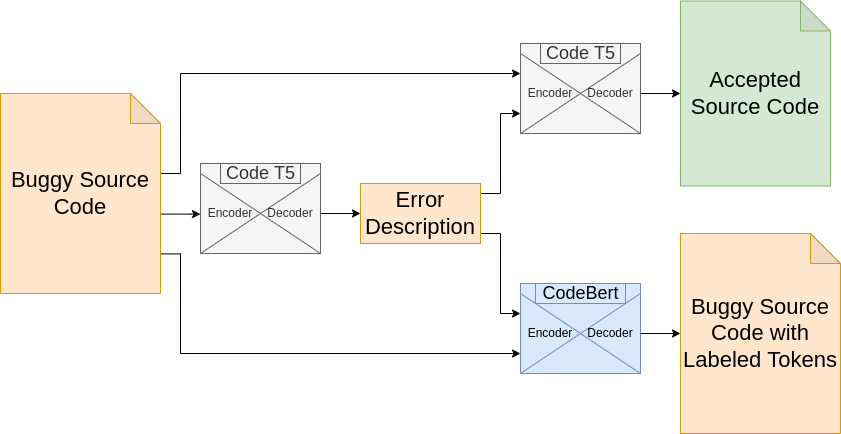
\includegraphics[width=\textwidth]{pics/bug-model.png}
  \caption{The bug detection and repair pipeline showing how the token labels and accepted source code files are generated.}
  \label{fig:solution1}
\end{figure}

\textbf{Bug Detection.} For the bug detection stage we have used the CodeT5 architecture. In our development we have used a model that was pretrained on the CodeSearchNet dataset to solve multiple tasks such as code summarization, code generation, code translation, code refinement, code defect detection or code clone detection tasks. This model uses a Byte-Pair Encoding (BPE) tokenizer. We fine tuned the CodeT5 model for the task of error description prediction on our BugNet dataset. We have used the preprocessed error messages from running the buggy submissions as supervision signal data. These error messages consist of the type of the error and a short description containing the location and features of the parts of the program involved in the crash.

\textbf{Bug Localization.} In the bug localization phase we have used the CodeBert architecture. The weights we have used for this model are also pretrained on the CodeSearchNet dataset. One of the best uses of this architecture is the token classification task, which involves predicting a class for each token in the input text. In our case we want to make a binary prediction for each token in our buggy source code. To fine tune the model to work for our task we have used both the buggy and accepted source code to generate the difference string. After we compare the buggy source code with the diff file we can generate ground truth labels for what changed from one submission to another. This information will represent the training data and what we want the model to be able to predict. The model will receive as input the error description, which is ideally predicted by the bug detection stage, and the buggy source code. The model will tokenize and concatenate the inputs and then generate a binary mask for the tokens. The bug localization task has the objective to help the programmer find the location of the bug predicted during the first phase of the pipeline.

\textbf{Bug Repair.} Since the bug repair task is very similar to a neural machine translation problem, we have decided to also use CodeT5 for this phase too. We have used the same pretrained weights as for the bug detection task and we have fine-tuned the model to be able to predict accepted source code from buggy source code. The model input consists of the error description and the buggy source code and will output a modified version of the original source code which should be able to be accepted in the competition. We have experimented with both generating the entire source code from scratch and also generating only the code that is labeled as buggy.

The ideal scenario for the bug detection and repair algorithm is having a single chunk bug prediction, identifying the buggy chunk and then using that information to predict a replacement for that part of the code. This means that we want to first localize the bug and then to generate an explanation and fix for it. In this way we can make use of large language models like Codex or ChatGPT to repair the bugs that we identify.

\section{Implementation}

To train and evaluate the models we have used the Kaggle GPU environment and the HuggingFace library. We have chosen the Kaggle environment over the Google Colab one because we were able to persist the dataset in a public repository, which does not require manual download each time the experiments are ran. On top of that, Kaggle offers 30 hours of GPU time per week for free tier.

The HuggingFace Transformers library is very popular for NLP tasks and it contains tools such as \textit{datasets}, which we used to load the data in a format which can be easily preprocessed after. Additionally, this library has access to a large collection of pretrained weights for different types of models, including models pretrained on the task of Masked Language Modeling (MLM) for Source Code, which is useful in our case. Predicting missing tokens in source code is not our goal, but using a model pretrained on a more general task can be beneficial. This is helpful because the model would understands, at some extent, the context it is going to be used in. To fine tune a model on a more specific task we will have to add new layers on top of the pretrained model (e.g to create a code classification model we may feed the input representation produced by the original model to a linear layer) and then training it on a new dataset made for that task.

\textbf{Bug Detection.} To fine tune the CodeT5 model on the task of bug detection we have used our BugNet dataset. From this dataset we have sampled only the source code files that had a return code different from zero. This means that the source code failed on the sample input and has an error description associated with it. The files with a return code of zero are also buggy, but due to limitations in the CodeNet dataset (it only contains the example input and output files) they do not have a crash associated with them, so there is no useful information to be learned. We also sample some of the accepted solutions and mark the error description with the text “Accepted” to indicate that a solution has no bugs. We then tokenize the buggy source code and the error descriptions with padding and truncation. Finally, we set the inputs as the buggy source code tokens and the labels as the error description tokens. For this task we used the datasets and the tokenizers tools from HuggingFace. In the training process we have used a batch size of 4, 500 warm up steps and a weight decay of 0.1 for one epoch. Because the error messages should indicate the problem in the source code we have used accuracy as the evaluation metric. To consider one prediction correct, all words in the predicted sentence must match the words from the ground truth sentence. In Table \ref{tab:experiments12} we show examples of what the Bug Detection model can output as error descriptions.

\begin{table}[H]\small\linespread{1}
\centering
\caption{Example of the predictions of the error descriptions for sample of source code from the test subset of CodeNetPy. Each cell contains the Source Code sample with the predicted description (selected some correct predictions).}
\label{tab:experiments12}
\begin{tabular}{p{15cm}}
\textbf{Source Code} \\
\hline
\begin{lstlisting}[language=Python]
s, t = map(input().split())
a, b = map(int, input().split())
t = input()
if s == t:
  print(str(a-1) + " " + str(b))
else:
  print(str(a) + " " + str(b-1))
\end{lstlisting}

TypeError: map() must have at least two arguments.

\\

\hline
\begin{lstlisting}[language=Python]
s,t=input().split()
a,b=map(int.input().split())
u=input()
print(a-1,b) if s==u else print(a,b-1)
\end{lstlisting}

AttributeError: type object 'int' has no attribute 'input'
\\

\hline
\begin{lstlisting}[language=Python]
s = input()
for i in len(s):
  print(x,end="")
\end{lstlisting}

TypeError: 'int' object is not iterable
\\
\end{tabular}
\end{table}

\textbf{Bug Localization.} For the bug localization task we have finetuned the CodeBert model on the CodeNetPy dataset. Since the model that we created takes as input both the error description and the source code, we have also filtered only the source code files that had a return code different from zero. We have also added accepted examples to the training set with an error description set as “Accepted”. To generate the input of the model we have used HuggingFace tokenizers and concatenated the error message with the source code. We have thus obtained a string of the form \textless{cls}\textgreater error description\textless{sep}\textgreater source code\textless{sep}\textgreater which we then tokenized with padding and truncation if needed. We have used Sequence Matcher on the buggy source code and the accepted source code to generate character level differences for the changes made between submissions. Then, we have mapped the changes to each token, such that if a character was changed in a token, then it is labeled as 1, otherwise it is labeled as 0. Because the output of the tokenizer contains tokens from the error description, source code and also padding, we have marked both the error and padding tokens with -100. This is needed such that the Cross Entropy Loss function will ignore them, and will only compute the error for the source code tokens, the ones that are labeled as 0 and 1. The algorithm is described in Table \ref{tab:experiments13}.

\begin{table}[H]\small\linespread{1}
\centering
\caption{The algorithm to label the tokens from the original source code based on the changed source code and error description.}
\label{tab:experiments13}
\begin{tabular}{p{10cm}}
\begin{lstlisting}
ranges = SequenceMatcher(original, changed)
tokens = tokenizer(error, original)

for each token in tokens do
    if token.from == original then
        if token.position in ranges then
            token.label = BUGGY
        else
            token.label = ACCEPTED
        fi
    else
        token.label = IGNORE
    fi
end
\end{lstlisting}
\\
\end{tabular}
\end{table}

We load the Token Classification model from microsoft/codebert-base and set the basic parameters for the trainer. We will also compute the metrics that will show precision, recall, f1 score and accuracy. For the task of bug localization, exact match score should be the best option, since we want to find the location of the specified bug in natural language.

To perform inference we will need the error description and the source code. The model will first tokenize the error and the source code, and then concatenate the tokens. After that, the model will output the logits for the buggy/non-buggy classes for each token in the input. We will only be interested in keeping only the labels for the PL tokens, and then to convert each pair of tokens back into words. Finally we can obtain the character labels from the word labels, using an inverse function from the preprocessing stage, that will take a word index and return all indices of the chars contained in that word. In Table \ref{tab:experiments14} are shown some examples of what the Bug Localization model can output as error labels for each token.

\begin{table}[H]\small\linespread{1}
\centering
\caption{Example of the predictions of the error label tokens for samples of source code from the test subset of CodeNetPy. Each cell contains the Source Code sample with the predicted labeled tokens (selected some correct predictions) colored in red.}
\label{tab:experiments14}
\begin{tabular}{p{15cm}}
\textbf{Source Code} \\
\hline
\begin{lstlisting}[escapeinside={(*}{*)}, language=Python]
s, t = input().split()
a, b = map(int, input().split())
u  (*\textcolor{red}{=}*) str(input())

if u = s:
  print(a-1, b)
else:
  print(a, b-1)
\end{lstlisting}

SyntaxError: invalid syntax
\\

\hline
\begin{lstlisting}[escapeinside={(*}{*)}, language=Python]]
S,T=map((*\textcolor{red}{input}*)().split()) 
A,B=map(int,input().split()) 
U=input() 
 
if U==S: 
  print(A-1) 
  print(B) 
else: 
  print(A) 
  print(B-1)
\end{lstlisting}

TypeError: map() must have at least two arguments.
\\

\hline
\begin{lstlisting}[escapeinside={(*}{*)}, language=Python]]
s,t = map(str,input().split()) 
a,b = map(int,input().split()) 
u = (*\textcolor{red}{int(input())}*)
if s == u: 
  print(a-1,b) 
else: 
  print(a,b-1)
\end{lstlisting}

ValueError: invalid literal for int() with base 10: 'red'
\\

\end{tabular}
\end{table}

\textbf{Bug Repair.} The bug repair stage is a task similar to neural machine translation. This task can be solved with a model such as T5. So in our implementation we used CodeT5 weights as we did for Bug Detection. For this phase we have used the buggy source code and error description as input and the accepted source code as output. We have also used the HuggingFace tokenizer to generate the inputs of the model. We concatenated the error message and the original source code and obtained \textless{cls}\textgreater error description\textless{sep}\textgreater source code\textless{sep}\textgreater and also tokenized the changed source code and obtained \textless{cls}\textgreater source code\textless{sep}\textgreater. As before, we have used padding and truncation. We have set the maximum truncation size to 512, which is enough for any of the tested source code files. We have set the labels of the input to be equal to the tokenized accepted source code. Finally we have set to ignore the tokens that come from padding for the labels. This way the model will compute the loss only for the tokens that are part of the changed source code. We have used the same parameters for training as for the Bug Detection task and also computed the accuracy.

To perform inference we will need the error description and the source code. The model will then predict the new source code based on the two inputs. In Table \ref{tab:experiments15} are shown some examples of what the Bug Repair model can output as source code for each buggy file.

\textbf{Masked BugRepair} Initially we considered bug repair as a machine translation task, so this means that the model had to generate the entire source code from the buggy source code. This was not the best method since it has the potential to introduce more bugs then before. So a better way is to use the bug localization results as a mask and then use the T5 for generation model to predict only the masked source code.  To fine tune the model we have generated masks in the locations of buggy source code and let the model predict the correct source code based on the rest of the code and the error description. This resulted in a much better accuracy then the machine translation approach.

\begin{table}[H]\small\linespread{1}
\centering
\caption{Examples of the predictions of the code repair for samples of source code from the test subset of CodeNetPy. Each cell contains the Source Code sample with the predicted buggy tokens colored in red and the ground truth source code colored in blue.}
\label{tab:experiments15}
\begin{tabular}{p{7.5cm} p{7.5cm}}
\textbf{Source Code} & \textbf{GT Source Code} \\
\hline
\begin{lstlisting}[escapeinside={(*}{*)}, language=Python]]
s,t=input().split() 
a,b=map(int,input().split()) 
u=input() 
if s==u: 
  print((*\textcolor{red}{s}*)-1 (*\textcolor{red}{t}*)) 
else: 
  print((*\textcolor{red}{s}*) (*\textcolor{red}{t}*)-1)
\end{lstlisting}

SyntaxError: invalid syntax & 
\begin{lstlisting}[escapeinside={(*}{*)}, language=Python]]
s,t=input().split() 
a,b=map(int,input().split()) 
u=input() 
if s==u: 
  print(s-1(*\textcolor{blue}{,}*) t) 
else: 
  print(s(*\textcolor{blue}{,}*) t-1)
\end{lstlisting}

SyntaxError: invalid syntax
\\

\hline
\begin{lstlisting}[escapeinside={(*}{*)}, language=Python]]
S,T = input().split()
A,B = (*\textcolor{red}{i}*)nt(*\textcolor{red}{(}*)input().split())
U = input()
if U == S:
  print(A-1,B)
elif U == T:
  print(A,B-1)
\end{lstlisting}

TypeError: int() argument must be a string, a bytes-like object or a number, not 'list' & 
\begin{lstlisting}[escapeinside={(*}{*)}, language=Python]]
S,T = input().split()
A,B = (*\textcolor{blue}{map(i}*)nt(*\textcolor{blue}{,}*) input().split())
U = input()
if U == S:
  print(A-1,B)
elif U == T:
  print(A,B-1)
\end{lstlisting}

TypeError: int() argument must be a string, a bytes-like object or a number, not 'list'
\\
\end{tabular}
\end{table}

\section{Quantitative Evaluation}

For the task of bug localization we have used two different evaluations, the first one is a token level comparison, shown in Table \ref{tab:experiments9}, and the second one is a document level comparison, shown in Table \ref{tab:experiments11}. The token level evaluation works by using the model to predict a label for each token and then using the test set to check if each label is correct. The second type of evaluation we used will decide if the source code is Accepted or not Accepted by checking if there are any buggy labels in the prediction. If the source code is bug free we label it accepted, otherwise we label it as not accepted. Then we check using the test set if each document is correctly classified.

\begin{table}[H]\small\linespread{1}
\centering
\caption{Quantitative results of the Bug Localization algorithm for token level predictions}
\label{tab:experiments9}
\begin{tabular}{p{4cm} l >{\raggedright\arraybackslash}p{2cm} >{\raggedright\arraybackslash}p{2cm} >{\raggedright\arraybackslash}p{2cm} >{\raggedright\arraybackslash}p{2cm}}
\textbf{Method} & \textbf{Accuracy} & \textbf{Precision} & \textbf{Recall} & \textbf{F1} \\
\hline
Decision Tree                  & 0.8765 & 0.2028 & 0.0092 & 0.0177 \\
\hline
CodeBert                  & \textbf{0.8990} & \textbf{0.6518} & \textbf{0.2554} & \textbf{0.3670} \\
\end{tabular}
\end{table}

\begin{table}[H]\small\linespread{1}
\centering
\caption{Quantitative results of the Bug Localization algorithm for document level predictions: Accepted vs non Accepted}
\label{tab:experiments11}
\begin{tabular}{p{4cm} l >{\raggedright\arraybackslash}p{2cm} >{\raggedright\arraybackslash}p{2cm} >{\raggedright\arraybackslash}p{2cm} >{\raggedright\arraybackslash}p{2cm}}
\textbf{Method} & \textbf{Accuracy} & \textbf{Precision} & \textbf{Recall} & \textbf{F1} \\
\hline
Decision Tree                  & 0.5270 & \textbf{0.5561} & 0.0898 & 0.1546 \\
\hline
CodeBert                  & \textbf{0.6536} & 0.3305 & \textbf{0.8582} & \textbf{0.4772} \\
\end{tabular}
\end{table}

Earlier we stated that our dataset contains 50\% accepted submissions and 50\% not accepted submissions. This means that if a model was to predict the label "accepted" for every input it would get an accuracy of 50\%. The model we used as a baseline for our research obtains a precision of 50\%. This means that half of the positive predictions of our model will be false positives, which makes it not much better than always predicting "accepted".

For the token level evaluation we are faced with the same problem. The model will be biased towards choosing "accepted" as the output label of most of the tokens. Analyzing the test set we obtained that 87\% of the tokens will have the label "accepted". From what we already know about accuracy and the results from Table \ref{tab:experiments7} we can confirm that this is the case for the Decision Tree Classifier model. The baseline model that uses Decision Trees is able to predict some of the tokens as buggy, but the model overfits on the training data and will predict "Accepted" most of the times. However, the CodeBert based model is able to predict better the buggy tokens. The model manages to find 1 in 4 buggy tokens in source code, but this type of localization is not covered in recent work. Current methods are able to identify 1 in 3 buggy files, which would not be a fair comparison since a file is considered buggy if it contains one buggy token. To make such a comparison we can look the recall for document level predictions. The baseline model has a very low recall, but this happens because it is biased to predicting "Accepted" for the tokens and the precision shows that with almost 50\% which is equal to the split of buggy and not buggy documents. On the other hand, CodeBert is able to identify over 3 in 4 buggy documents, but it also has a high false positive rate, since the precision is small. The results are similar to related work experiments. In most cases language models trained on source code tend to have a high false positive rate when identifying bugs.

\begin{table}[H]\small\linespread{1}
\centering
\caption{Quantitative results of the Bug Detection algorithm: Full Description Text Generation}
\label{tab:experiments16}
\begin{tabular}{p{4cm} l >{\raggedright\arraybackslash}p{2cm} >{\raggedright\arraybackslash}p{2cm} >{\raggedright\arraybackslash}p{2cm} >{\raggedright\arraybackslash}p{2cm}}
\textbf{Method} & \textbf{Accuracy} \\
\hline
CodeT5                  & 0.162  \\
\hline
CodeT5 + Beam Size 5    & 0.218 \\
\hline
CodeT5 + Beam Size 10   & 0.225 \\
\hline
CodeT5 + Beam Size 50   & \textbf{0.256} \\
\end{tabular}
\end{table}

\begin{table}[H]\small\linespread{1}
\centering
\caption{Quantitative results of the Bug Detection algorithm: Error Class Text Generation}
\label{tab:experiments17}
\begin{tabular}{p{4cm} l >{\raggedright\arraybackslash}p{2cm} >{\raggedright\arraybackslash}p{2cm} >{\raggedright\arraybackslash}p{2cm} >{\raggedright\arraybackslash}p{2cm}}
\textbf{Method} & \textbf{Accuracy} & \textbf{Precision} & \textbf{Recall} & \textbf{F1} \\
\hline
T5-base + Beam Size 50  & 0.038  & -  & -  & -  \\
\hline
CodeT5                  & 0.2090  & 0.2259  & 0.9675  & 0.3663  \\
\hline
CodeT5 + Beam Size 5    & 0.2560  & 0.2633  & 0.9733  & 0.4145  \\
\hline
CodeT5 + Beam Size 10   & 0.2690  & 0.2730  & 0.9746  & 0.4266  \\
\hline
CodeT5 + Beam Size 50   & \textbf{0.2770}  & \textbf{0.2789}  & \textbf{0.9753}  & \textbf{0.4338} \\
\end{tabular}
\end{table}

To evaluate the Error Description message generation we have used the exact match metric. We made this decision because we want that the error messages identically match the training. The error messages work both as a class and extra information for where and why the bug was predicted. The analysis is done at the word level, such that we compare all sentences. For example if the model predicts an error description of length 10 words and it differs from the ground truth by one word, then the accuracy of it would be 90\%. The results show an accuracy of 25\% for the CodeT5 model in Table \ref{tab:experiments16}. In the qualitative results we found that the model will usually predict correctly the error class but will sometimes make small mistakes in the full description. The result of predicting only the first word of the description is shown in Table \ref{tab:experiments17}.

\begin{table}[H]\small\linespread{1}
\centering
\caption{Quantitative results of the Bug Repair algorithm: Source Code Generation}
\label{tab:experiments18}
\begin{tabular}{p{4cm} l >{\raggedright\arraybackslash}p{2cm} >{\raggedright\arraybackslash}p{2cm} >{\raggedright\arraybackslash}p{2cm} >{\raggedright\arraybackslash}p{2cm}}
\textbf{Method} & \textbf{Accuracy} \\
\hline
CodeT5                              & 0.013 \\
\hline
CodeT5 + Beam Size 5                & 0.019 \\
\hline
CodeT5 + Beam Size 10               & 0.021 \\
\hline
CodeT5 + Beam Size 50               & 0.025 \\
\hline
CodeT5 + Beam Size 50 + Masked      & \textbf{0.366} \\
\end{tabular}
\end{table}

Finally we have evaluated the Bug Repair model from our pipeline on the same test dataset as for the other two components. To evaluate this model we have considered that for a prediction to be considered correct, the output of the model has to be identical to the ground truth source code. The model will be input the buggy source code and the error description message and will output the new source code using the CodeT5 pretrained model. The results of the evaluation are in Table \ref{tab:experiments18}.

Models designed purely for code generation from natural language description reach an accuracy of 30\%. However, such models are trained on very large collections of data such as GitHub Copilot. Additionally, some of these models are able to generate multiple predictions and the accuracy is increased if any of the predictions are correct. Our Code Generation model is implemented in a greedy way. It will only choose the argmax tokens that are generated. By utilizing a beam search algorithm for generating the predictions we can increase the accuracy of the Code T5 model to reach a major improvement over the greedy decoding. The beam search algorithm will choose the top K predictions that maximize the likelihood of the source code being not buggy. To compute the number of accepted cases using such an approach it is enough to have a single correct prediction among the K proposed solutions.

We have also found that using pretrained weights as a starting point for the Roberta and T5 models improved the performance of the algorithm. Fine tuning on our BugNet Dataset improved the models results from an accuracy of 3.8\% to 27.7\% in case of bug detection, showed in Table \ref{tab:experiments17}. However, during analysis we have observed that we cannot obtain as good results if we would train from scratch on our dataset alone. Using models pretrained on a large collection of source code, such as CodeSearchNet, proved to be essential for our tasks.

\chapter{Additional examples}

In Table \ref{tab:appendices1} we can see some additional examples where the CodeT5 Bug Detection model did not find the ground truth error descriptions. However, this are some interesting results nonetheless. In the first example we can see that the model predicted that the function object from the first line is not iterable, which is a legitimate response, however, looking at the entire instruction, the problem arises because of the assignment and that is what the Python interpreter is going to have trouble with. In the second example, the bug detection algorithm actually found a correct problem, the fact that the int function cannot be applied on a list object. But in the same manner as before, the interpreter will read the instruction from left to right and find the map function call first, which should have two arguments, and stop there throwing an error. For the third and last example in the table, the problem arises from the input format, not the source code, so predicted that the solution is correct is to be expected. The model would not be able to take into account what the input can be unless it has access to the problem statement or some examples of input and output.

\begin{table}[H]\small\linespread{1}
\centering
\caption{Additional examples of the predictions of the error descriptions for sample of source code from the test subset of CodeNetPy. Each cell contains the Source Code sample with the predicted description and the correct description.}
\label{tab:appendices1}
\begin{tabular}{p{15cm}}
\textbf{Source Code} \\
\hline
\begin{lstlisting}[language=Python]
a,b = input().split
c,d = map(int,input().split())
e = input()

if a == e:
  print("{} {}".format(c-1,d))
else:
  print("{} {}".format(c,d-1))
\end{lstlisting}

TypeError: 'builtin\_function\_or\_method' object is not iterable

TypeError: cannot unpack non-iterable builtin\_function\_or\_method object

\\

\hline
\begin{lstlisting}[language=Python]
s, t = map(input().split())

a, b = map(int(input().split()))

u = input()

if s == u:
    print(a - 1, b)
elif t == u:
    print(a, b - 1)
\end{lstlisting}

TypeError: int() argument must be a string, a bytes-like object or a number

TypeError: map() must have at least two arguments.

\\

\hline
\begin{lstlisting}[language=Python]
[H, A] = [int(i) for i in input().split()]
t = 0
if H/A != int(H/A):
    t = 1
print(int(H/A) + t)
\end{lstlisting}

Accepted

ValueError: invalid literal for int() with base 10: 'red'
\\
\end{tabular}
\end{table}

In Table \ref{tab:appendices2} we can see some additional examples where the CodeBert Bug Localization model did not find the ground truth token labels. In the first example we can see that the model predicted as buggy the tokens that are related to the assigment operation. However, a correct solution should convert the string into a list and then at the end it should convert it back into a string. In the second example, the model predicted well that the problem appears on the second line, however it also predicted some false positive.

\begin{table}[H]\small\linespread{1}
\centering
\caption{Additional examples of the predictions of the error label tokens for samples of source code from the test subset of CodeNetPy. Each cell contains the Source Code sample with the predicted labeled tokens colored in red. The column on the right will show the ground truth labels in blue.}
\label{tab:appendices2}
\begin{tabular}{p{7.5cm} p{7.5cm}}
\textbf{Source Code} & \textbf{GT Source Code} \\
\hline
\begin{lstlisting}[escapeinside={(*}{*)}, language=Python]
s = input() 
for i in range(len(s)): 
  s[i] (*\textcolor{red}{= "x}*)" 
print(s)
\end{lstlisting}

TypeError: 'str' object does not support item assignment & 
\begin{lstlisting}[escapeinside={(*}{*)}, language=Python]
s = input((*\textcolor{blue}{)}*)
for i in range(len(s)): 
  (*\textcolor{blue}{s[i]}*) = "x" 
print((*\textcolor{blue}{s}*))
\end{lstlisting}

TypeError: 'str' object does not support item assignment
\\

\hline
\begin{lstlisting}[escapeinside={(*}{*)}, language=Python]
S,T = input().split() 
A,B = (*\textcolor{red}{int(}*)input().split()) 
U = (*\textcolor{red}{input}*)() 
if U == S: 
  	print(A-1,B) 
elif U == T: 
    print(A,B-1) 
\end{lstlisting}

TypeError: int() argument must be a string, a bytes-like object or a number, not 'list' & 
\begin{lstlisting}[escapeinside={(*}{*)}, language=Python]
S,T = input().split() 
A,B = (*\textcolor{blue}{int(}*)input().split()) 
U = input() 
if U == S: 
  	print(A-1,B) 
elif U == T: 
    print(A,B-1) 
\end{lstlisting}

TypeError: int() argument must be a string, a bytes-like object or a number, not 'list'
\\

\end{tabular}
\end{table}

From the additional experiments made on the bug detection model we have found that the precision of the model to generate meaningful error messages increases with the number of beams used in decoding the output. In Table \ref{tab:appendices3} and Table \ref{tab:appendices4} we found that by using 5 possible outputs, the model was able to correctly predict 2 out of 4 bugs, while before it wasn't able to predict any of them correctly. This is a great improvement for our pipeline but it can lead to generating very many possible corrections for the buggy source code, which can be challenging for a developer to choose from without help from testing tools.

\begin{table}[H]\small\linespread{1}
\centering
\caption{Additional examples of the predictions of the error descriptions for sample of source code from the test subset of CodeNetPy. In this table is shown the output of a beam search algorithm. The correct answer is in bold, and if the model predicted the right answer in underline and bold. Each cell contains the Source Code sample with the predicted description and the correct description.}
\label{tab:appendices3}
\begin{tabular}{p{15cm}}
\textbf{Source Code} \\
\hline
\begin{lstlisting}[language=Python]
a,b = input().split
c,d = map(int,input().split())
e = input()

if a == e:
  print("{} {}".format(c-1,d))
else:
  print("{} {}".format(c,d-1))
\end{lstlisting}

TypeError: 'builtin\_function\_or\_method' object is not iterable

TypeError: unsupported operand type(s) for -: 'builtin\_function\_or\_

TypeError: can only concatenate str (not "builtin\_function\_or\_method") to

AttributeError: 'builtin\_function\_or\_method' object has no attribute'split

TypeError: 'builtin\_function\_or\_method' object is not subscriptable

\textbf{TypeError: cannot unpack non-iterable builtin\_function\_or\_method object}

\\

\hline
\begin{lstlisting}[language=Python]
s, t = map(input().split())

a, b = map(int(input().split()))

u = input()

if s == u:
    print(a - 1, b)
elif t == u:
    print(a, b - 1)
\end{lstlisting}

TypeError: int() argument must be a string, a bytes-like object or a number

\underline{\textbf{TypeError: map() must have at least two arguments.}}

TypeError: int() argument must be a string or a number, not 'list'

TypeError: 'int' object is not iterable

ValueError: invalid literal for int() with base 10: 'apple'

\\

\end{tabular}
\end{table}

\begin{table}[H]\small\linespread{1}
\centering
\caption{Additional examples of the predictions of the error descriptions for sample of source code from the test subset of CodeNetPy. In this table is shown the output of a beam search algorithm. The correct answer is in bold, and if the model predicted the right answer in underline and bold. Each cell contains the Source Code sample with the predicted description and the correct description.}
\label{tab:appendices4}
\begin{tabular}{p{15cm}}
\textbf{Source Code} \\

\hline
\begin{lstlisting}[language=Python]
[H, A] = [int(i) for i in input().split()]
t = 0
if H/A != int(H/A):
    t = 1
print(int(H/A) + t)
\end{lstlisting}

Accepted

TypeError: unsupported operand type(s) for /: 'int' and'str'

TypeError: unsupported operand type(s) for /:'str' and 'int'

ValueError: not enough values to unpack (expected 2, got 1)

ValueError: invalid literal for int() with base 10: '2 5'

\textbf{ValueError: invalid literal for int() with base 10: 'red'}

\\

\hline
\begin{lstlisting}[language=Python]
s = input()
for i in range(len(s)):
  s[i] = "x"
print(s)
\end{lstlisting}

Accepted

TypeError:'str' object cannot be interpreted as an integer

TypeError: object of type'str' has no len()

\underline{\textbf{TypeError:'str' object does not support item assignment}}

TypeError: 'int' object is not iterable

\\

\end{tabular}
\end{table}

Experimenting with the source code generation model we have encountered examples such as in Table \ref{tab:appendices5} that show that using only the buggy source code and error description would not be enough to be able to provide the user with a correct submission. We have found that even if the model is able to fix the source code it is also very probable that it will encounter false positives and break existing code. In this case we should also make use of our generated token labels as a type of mask such that the model is able to only modify what is predicted as buggy. We have found that the CodeBert model is much more accurate at localizing the buggy tokens than the CodeT5 model during the generation process. We have also found examples where the source code cannot convey enough context to what task it is trying to achieve, especially in very short scripts. This problem might be solved by utilizing the problem statement, or comments from the user in the source code generation task.

\begin{table}[H]\small\linespread{1}
\centering
\caption{Examples of the predictions of the code repair for samples of source code from the test subset of CodeNetPy. Each cell contains the Source Code sample with the predicted source code tokens colored in red and the ground truth source code colored in blue.}
\label{tab:appendices5}
\begin{tabular}{p{7.5cm} p{7.5cm}}
\textbf{Predicted Source Code} & \textbf{GT Source Code} \\
\hline
\begin{lstlisting}[escapeinside={(*}{*)}, language=Python]
s, t = (*\textcolor{red}{list(map(int, }*)input().split()(*\textcolor{red}{))}*)
a, b = (*\textcolor{red}{[0, 0]}*)
u = input()
if s == u:
    a = a - 1
(*\textcolor{red}{elif t == -1 or a \textless 0 or b \textless0:}*)
    (*\textcolor{red}{print(0)}*)
(*\textcolor{red}{else: print(a * b, (a + b) * 2 )}*)
\end{lstlisting}

TypeError: map() must have at least two arguments. & 
\begin{lstlisting}[escapeinside={(*}{*)}, language=Python]
s, t = (*\textcolor{blue}{map(str,}*)input().split()(*\textcolor{blue}{)}*)
a, b = map(int, input().split())
u = input()
if s == u:
    a = a - 1
else:
    b = b -1
print(a, b)
\end{lstlisting}

TypeError: map() must have at least two arguments.
\\

\hline
\begin{lstlisting}[escapeinside={(*}{*)}, language=Python]
s = input()
print((*\textcolor{red}{len(s) * 2}*))
\end{lstlisting}

NameError: name 'x' is not defined & 
\begin{lstlisting}[escapeinside={(*}{*)}, language=Python]
s = input()
print((*\textcolor{blue}{"}*)x(*\textcolor{blue}{"}*) * len(s))
\end{lstlisting}

NameError: name 'x' is not defined
\\

\hline
\begin{lstlisting}[escapeinside={(*}{*)}, language=Python]
s = input()
(*\textcolor{red}{x = int(s)}*)
print((*\textcolor{red}{x * x}*))
\end{lstlisting}

NameError: name 'x' is not defined & 
\begin{lstlisting}[escapeinside={(*}{*)}, language=Python]
s = input()
print((*\textcolor{blue}{"}*)x(*\textcolor{blue}{"}*) * len(s))
\end{lstlisting}

NameError: name 'x' is not defined
\\

\hline
\begin{lstlisting}[escapeinside={(*}{*)}, language=Python]
s = input()
print((*\textcolor{red}{int(s) ** 3}*))
\end{lstlisting}

NameError: name 'x' is not defined & 
\begin{lstlisting}[escapeinside={(*}{*)}, language=Python]
s = input()
print((*\textcolor{blue}{"}*)x(*\textcolor{blue}{"}*) * len(s))
\end{lstlisting}

NameError: name 'x' is not defined
\\
\end{tabular}
\end{table}

A pipeline that considers the buggy source code with labeled tokens in the source code generation process is presented in Table \ref{fig:appendices1}. This new pipeline would also use human input text for a better error message generation. This input text would be given as natural language, either in the form of a problem statement or as a comment in the source code, similar to how many such tools work in IDEs. The input text would be then paired with the buggy source code and fed into the model, to generate an improved error description. Then we can continue to use the source code and error description to find the buggy tokens. Finally we would use the problem description, the error description and the source code to generate a prediction for the accepted source code, while attending to the buggy tokens we found in the bug localization stage. This process would alleviate the problem of the model changing source code that is not predicted as buggy, and also improving the context of what the goal of the given code is.

\begin{figure}[H]
\centering
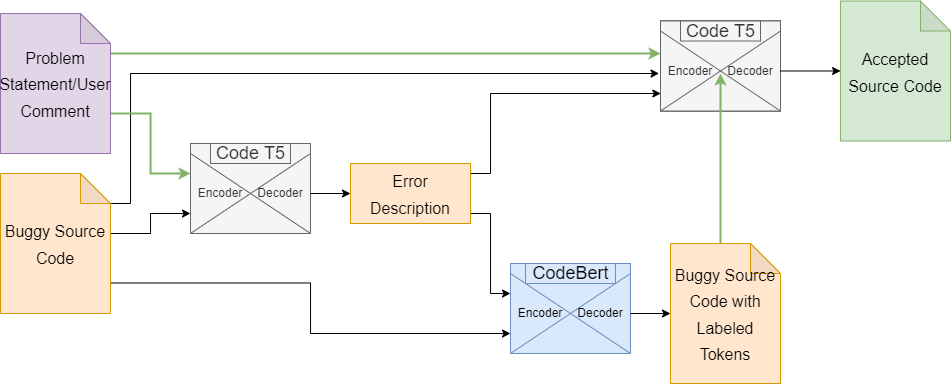
\includegraphics[width=\textwidth]{pics/bug-model-future.png}
  \caption{The bug detection and repair pipeline for future work that includes the problem statement or the user comments and also takes into consideration the labeled buggy tokens in the process of source code generation.}
  \label{fig:appendices1}
\end{figure}

\chapter{Codex examples}

\textbf{Example 1}

In the first example, Codex manages to solve the problem, however, the ground truth solution was not identical. This is one of the issues that led to low accuracy on the API experiment.

\textit{Original Source Code}

\begin{lstlisting}[escapeinside={(*}{*)}, language=Python]
num = [int(input()) for i in range(10)]
num.sort(reverse=True)
(*\textcolor{red}{for i in range[0:3]:}*)
    print(num[i])
\end{lstlisting}

\textit{Codex Prediction}

\begin{lstlisting}[escapeinside={(*}{*)}, language=Python]
(*\textcolor{red}{for i in range(0, 3):}*)
\end{lstlisting}

\textit{Ground Truth}

\begin{lstlisting}[escapeinside={(*}{*)}, language=Python]
(*\textcolor{blue}{for i in range(3):}*)
\end{lstlisting}

\textbf{Example 2}

Another problem that can arise is the incorrect use of whitespaces. This issue can be managed at some extent compared to the previous one. We can try to remove the whitespace and compare only the important characters. However, in languages like Python, where whitespaces are part of the syntax this is not possible.

\textit{Original Source Code}

\begin{lstlisting}[escapeinside={(*}{*)}, language=C++]
#include <bits/stdc++.h> 
using namespace std; 
 
int main() { 
  (*\textcolor{red}{vector\textless{int}\textgreater mountain;}*)
  for (int i = 0; i < 10; i++) { 
    cin >> mountain.at(i); 
  } 
  sort(mountain.begin(), mountain.end()); 
  reverse(mountain.begin(), mountain.end()); 
 
  for (int i = 0; i < 3; i++) { 
    cout << mountain.at(i) << endl; 
  } 
}
\end{lstlisting}

\textit{Codex Prediction}

\begin{lstlisting}[escapeinside={(*}{*)}, language=C++]
(*\textcolor{red}{vector\textless{int}\textgreater mountain(10);}*)
\end{lstlisting}

\textit{Ground Truth}

\begin{lstlisting}[escapeinside={(*}{*)}, language=C++]
(*\textcolor{blue}{••vector\textless{int}\textgreater mountain(10);}*)
\end{lstlisting}

\textbf{Example 3}

In this example we can see how the Codex model sometimes is outputting natural language indication of the actions that the user needs to take. This can be the hardest problem to solve from the ones presented so far. One option would be to generate more answers from Codex, until one of them is just code. We can try to increase the temperature and have more randomness. For example, we can ask for 10 predictions and if one is correct we consider the run accurate.

\textit{Original Source Code}

\begin{lstlisting}[escapeinside={(*}{*)}, language=C++]
#include <algorithm> 
#include <iostream> 
using namespace std; 
int main() { 
  int a[10]; 
  for (int i = 0; i < 10; i++) { 
    cin >> a[i]; 
  } 
  sort(a, a + 10); 
  (*\textcolor{red}{for (int i = 9; i \textgreater 6; i++) \{}*)
    cout << a[i] << endl; 
  } 
  return 0; 
}
\end{lstlisting}

\textit{Codex Prediction}

\begin{lstlisting}[escapeinside={(*}{*)}, language=C++]
(*\textcolor{red}{change i \textgreater 6 to i \textgreater= 6}*)
\end{lstlisting}

\textit{Ground Truth}

\begin{lstlisting}[escapeinside={(*}{*)}, language=C++]
(*\textcolor{blue}{  for (int i = 9; i \textgreater 6; i--) \{}*)
\end{lstlisting}

\textbf{Example 4}

Just an example where Codex was able to find the correct solution.

\textit{Original Source Code}

\begin{lstlisting}[escapeinside={(*}{*)}, language=C++]
input()

a = list(map(int, input().split()))

s = 0

(*\textcolor{red}{for i in len(a):}*)
    s = s + i

print(min(a), max(a), s)
\end{lstlisting}

\textit{Codex Prediction}

\begin{lstlisting}[escapeinside={(*}{*)}, language=C++]
(*\textcolor{blue}{for i in a:}*)
\end{lstlisting}

\textit{Ground Truth}

\begin{lstlisting}[escapeinside={(*}{*)}, language=C++]
(*\textcolor{blue}{for i in a:}*)
\end{lstlisting}

\end{appendices}
\end{document}